% This template can serve as a starting point for your BSc thesis. You are allowed to modify it as long as you adhere to the requirements from the Thesis Manual.
\documentclass[a4paper,11pt]{article}

% FILL OUT THE DETAILS BELOW:
\author{
\begin{tabular}{cc}
Ruben Dunnewolt (661890) & Joost Fitton (659382) \\
Luuk Jille (703714)     & Kevin Smit (707087)
\end{tabular}
}
\title{The Post-1994 Breakdown of Equity Premium Combination Forecasts:
A Variance Decomposition Approach}
% \date{An optional custom date, the default is today}
\newcommand{\program}{Econometrics \& Operations Research}
\newcommand{\supervisor}{Sam van Meer}

\usepackage[british]{babel} % Use British English
\usepackage[onehalfspacing]{setspace} % Increase line spacing
\usepackage[margin=2.5cm]{geometry} % Modify margins
\usepackage{graphicx,booktabs} % Packages for images and tables
\usepackage[authoryear]{natbib} % APA-style author-year citations

% ADD YOUR OWN PACKAGES HERE
\usepackage{array}
\usepackage{threeparttable}
\usepackage{siunitx}
\usepackage{amsmath,amssymb,amsfonts}
\usepackage[counterclockwise]{rotating}
\usepackage{hyperref}
\usepackage{float}
\usepackage[T1]{fontenc}
\usepackage{titlesec}
\usepackage{microtype}
\usepackage{enumitem}
\usepackage{subcaption}
\usepackage{appendix}

\begin{document}

\begin{titlepage}
\makeatletter
\begin{center}
	\textsc{Erasmus University Rotterdam}
	\par \textsc{Erasmus School of Economics}
	\par Seminar in Investing \program

	\vspace{0.5cm} \hrule height .08em \bigskip
	\par\huge\@title\bigskip
	\par\Large\@author\bigskip
	\hrule height .08em\normalsize
	
	\vspace{1cm} % small controlled space instead of stretch

\includegraphics[width=\textwidth,height=0.15\textheight,keepaspectratio]{eur}

\vspace{0.8cm}
\begin{tabular}{ll}
	
		\toprule
		Supervisor: & \supervisor\\
		Date final version: & \@date\\
		\bottomrule
	\end{tabular}
    \vspace{0.4cm}
\begin{abstract}
\noindent \citet{denkloffler2024} document a sharp post-1994 deterioration
in equity premium combination forecast performance, attributing it to
rising forecast error correlations, but do not identify what drives the
deterioration. We decompose the forecast error covariance matrix into
three components, a return-variance term, a forecast--return
cross-covariance term, and a forecast covariance term, and show empirically that the deterioration is driven almost entirely by a
collapse in the forecast--return cross-covariance component, with
negligible contributions from the other two. The collapse is homogeneous
across the predictor set rather than concentrated in individual predictors.
We then evaluate four methodologically distinct remedies: two that
restructure combination weights (scaled PCA and discounted MSFE) and two
that localise the individual predictive regressions (rolling-window OLS
and discounted OLS). None consistently outperforms the historical average
post-1994 in either statistical or economic terms. The convergence of
failure across these methodologically independent approaches confirms
that the breakdown reflects a fundamental misalignment between
macroeconomic predictors and realised returns rather than a failure of
combination or estimation design. Structural break tests reinforce this
interpretation: the deterioration does not coincide with a single sharp
break but unfolds gradually through the sample.
\end{abstract}
\end{center}
\makeatother

\end{titlepage}

% =====================================================================
\section{Introduction}\label{sec:intro}
% =====================================================================

\citet{goyalwelch2008} conduct an exhaustive examination of macroeconomic
predictors and find that most fail to beat the historical average in
out-of-sample evaluation. \citet{campbellthompson2008} refine this
assessment by imposing sign restrictions on predictive coefficients and
find positive but modest out-of-sample $R^{2}$ values for several
predictors. These conflicting findings motivate the combination approach
of \citet{rsz2010}, who show that, even though individual predictors fail
the Goyal--Welch test, their equal-weighted combination dominates the
historical average both statistically and economically. The intuition is
straightforward: if individual forecast errors are at least partially
independent, averaging across models reduces variance. Equal-weighted
combination, despite its simplicity, is difficult to beat in practice
\citep{timmermann2006}.

\citet{denkloffler2024} re-examine this result using data through 2022 and
show that the out-of-sample performance of combination forecasts has
become insignificant or negative in recent subsamples, with the sharpest
deterioration occurring after 1994. They attribute this pattern to
forecast errors becoming increasingly correlated over time, which directly
erodes the diversification gains on which combination forecasts rely.
Their result is diagnostic rather than explanatory: it identifies
\textit{that} forecast errors have become more correlated, but not
\textit{why}, nor which component of the forecast error covariance matrix
is responsible for the deterioration. That gap is the motivation for this
paper.

Our contribution is threefold. \textit{First}, we develop an economically
interpretable decomposition of the forecast error covariance matrix into
three components, a return-variance term, a forecast--return
cross-covariance term, and a forecast covariance term, and show
empirically that the post-1994 deterioration is driven almost entirely by
a collapse in the forecast--return cross-covariance component. The
return-variance and forecast covariance components remain stable across
subperiods, and the collapse in forecast--return correlation is
homogeneous across the predictor set rather than concentrated in a few
predictors: individual predictor--return correlations fall together rather
than diverging. This diagnosis pinpoints which part of the covariance
structure breaks down and rules out the two leading competing
explanations, namely rising predictor co-movement and rising return
variance.

\textit{Second}, we systematically evaluate four methodologically distinct
remedies, each targeting a different plausible failure mode implied by the
diagnosis. Two act at the combination level, scaled PCA
\citep[sPCA,][]{huang2022scale} and discounted-MSFE combination
\citep{StockWatson2004}, and two at the estimation level, rolling-window
and discounted OLS. None of the four consistently outperforms the
historical average post-1994, in either statistical ($R^{2}_{OS}$) or
economic (CER) terms.

\textit{Third}, we argue that the convergence of failure across these
methodologically independent approaches is itself the central empirical
finding. Sophisticated combination design, adaptive weighting, and
localised estimation all fail in the same way, which confirms that the
problem lies in the predictor--return signal itself rather than in
combination or estimation design. Two pieces of evidence support this
interpretation. DMSFE weights remain essentially equal throughout the
sample, the effective number of active predictors stays at roughly~$N$
--- which confirms that the deterioration is homogeneous rather than
predictor-specific. Structural break tests indicate that the deterioration
does not coincide with a single sharp break but unfolds gradually: sup-F
and Bai--Perron tests on the forecast errors of the $1/N$ combination
identify multiple breaks spread through the sample rather than a discrete
shift around 1994.

Taken together, these results reframe the \citet{denkloffler2024}
finding: the post-1994 deterioration is not a combination-design problem.
It reflects a fundamental weakening of the predictor--return relationship
that no reweighting or cutoff scheme can recover. An implication for
future work is that improving equity premium forecasts is likely to
require modelling structural change in the predictors themselves, or
identifying alternative signal sources entirely, rather than further
refinements to combination methodology.

The rest of the paper is organised as follows.
Section~\ref{sec:decomposition} introduces the forecast error
decomposition, defines the diagnostic statistics, and presents the
diagnostic evidence, including structural break tests.
Section~\ref{sec:methods} describes the four forecasting methods and the
benchmarks. Section~\ref{sec:data} describes the data.
Section~\ref{sec:results} reports the empirical results,
organised by question rather than by method.
Section~\ref{sec:conclusion} concludes.

% =====================================================================
\section{Forecast Error Decomposition and Diagnostic Evidence}\label{sec:decomposition}
% =====================================================================

This section develops the decomposition of the forecast error covariance
matrix that is the theoretical core of the paper, and presents the
empirical diagnostic evidence that identifies which component drives the
post-1994 deterioration.

\subsection{Decomposition of the Forecast Error Covariance Matrix}\label{subsec:decomposition-theory}

Let $r_{t+1}$ denote the equity premium at time $t+1$ and $\mathcal{F}_t$
the information set available at time~$t$. For each predictor
$i = 1, \ldots, N$, we consider a forecast $\hat{r}_{i,t+1}$ of $r_{t+1}$
based on $\mathcal{F}_t$, obtained from a bivariate predictive regression
estimated recursively. We collect the $N$ forecasts in the vector
$\hat{\mathbf{r}}_{t+1} = (\hat{r}_{1,t+1}, \ldots, \hat{r}_{N,t+1})'$ and
the corresponding forecast errors $e_{i,t+1} = r_{t+1} - \hat{r}_{i,t+1}$
in $\mathbf{e}_{t+1}$, with covariance matrix $\Sigma_e$.

Applying the law of total variance
$\mathrm{Var}(r_{t+1}) =
\mathbb{E}[\mathrm{Var}(r_{t+1} \mid \mathcal{F}_t)] +
\mathrm{Var}(\mathbb{E}[r_{t+1} \mid \mathcal{F}_t])$ to the realised
equity premium, the covariance matrix of forecast errors decomposes as
\begin{equation}\label{eq:ltv-decomp}
    \Sigma_e =
    \underbrace{\mathbb{E}\!\left[\mathrm{Var}(r_{t+1} \mid \mathcal{F}_t)
        \right]\iota\iota'}_{\text{common-equity component}}
    \;+\;
    \underbrace{\mathrm{Var}\!\left(\mathbb{E}[r_{t+1} \mid \mathcal{F}_t]
        \,\iota - \hat{\mathbf{r}}_{t+1}\right)}_{\text{cross-forecast component}},
\end{equation}
where $\iota$ is the $N \times 1$ vector of ones. The first term captures
the part of return variation that is unpredictable given
$\mathcal{F}_t$; because the forecasts $\hat{\mathbf{r}}_{t+1}$ are
$\mathcal{F}_t$-measurable, they do not appear in it. Since every forecast
error is subject to the same unpredictable return shock, this term enters
every element of $\Sigma_e$ with a coefficient of one, reflected by the
$\iota\iota'$ structure.

To expand the cross-forecast component, we apply the standard variance
expansion, yielding five terms:
\begin{equation}\label{eq:cross-forecast-expand-resize}
\resizebox{\textwidth}{!}{$
    \Sigma_e =
    \underbrace{\mathbb{E}[\mathrm{Var}(r_{t+1} \mid \mathcal{F}_t)]
        \iota\iota'}_{\text{(i)}}
    + \underbrace{\mathrm{Var}(\mathbb{E}[r_{t+1} \mid \mathcal{F}_t])
        \iota\iota'}_{\text{(ii)}}
    - \underbrace{\iota\,\mathrm{Cov}(\mathbb{E}[r_{t+1} \mid \mathcal{F}_t],
        \hat{\mathbf{r}}_{t+1})'}_{\text{(iii)}}
    - \underbrace{\mathrm{Cov}(\mathbb{E}[r_{t+1} \mid \mathcal{F}_t],
        \hat{\mathbf{r}}_{t+1})\,\iota'}_{\text{(iv)}}
    + \underbrace{\mathrm{Var}(\hat{\mathbf{r}}_{t+1})}_{\text{(v)}}.
$}
\end{equation}

To understand which components can be reduced, write the realised return
as
\begin{equation}
    r_{t+1} = F(\mathcal{F}_t) + \varepsilon_{t+1},
\end{equation}
where $F(\mathcal{F}_t) = \mathbb{E}[r_{t+1} \mid \mathcal{F}_t]$ is the
true conditional expectation and $\varepsilon_{t+1}$ is the innovation,
satisfying $\mathbb{E}[\varepsilon_{t+1} \mid \mathcal{F}_t] = 0$.
$F(\mathcal{F}_t)$ is the part of return variation that is in principle
predictable; $\varepsilon_{t+1}$ is the part that no model can recover.

Term~(i), the \textit{innovation variance}
$\mathbb{E}[\mathrm{Var}(r_{t+1} \mid \mathcal{F}_t)] =
\mathrm{Var}(\varepsilon_{t+1})$, is irreducible by construction:
$\varepsilon_{t+1}$ is orthogonal to every $\mathcal{F}_t$-measurable
quantity and therefore to every forecast $\hat{r}_{i,t+1}$. The same shock
hits every forecast error simultaneously and with equal force, reflected
in the $\iota\iota'$ structure.

A caveat on the label ``irreducible.'' In population, term~(i) is fixed:
no forecaster can recover $\varepsilon_{t+1}$ from $\mathcal{F}_t$. In
practice, we approximate $F(\mathcal{F}_t)$ with bivariate regressions on
the Goyal--Welch predictor set, and the boundary between reducible and
irreducible in our decomposition is drawn by \emph{that} set. If a richer
predictor universe were available, some of what we assign to term~(i)
empirically would shift into term~(ii), it is reducible in principle,
just not by our instruments. Our estimates of the innovation variance
should therefore be read as an upper bound on what the Goyal--Welch set
can explain, not as a characterisation of fundamental unpredictability
of the equity premium.

Term~(ii), the \textit{conditional mean variance}
$\mathrm{Var}(\mathbb{E}[r_{t+1} \mid \mathcal{F}_t])$, represents the part
of return variation that is predictable in principle. A forecaster who
knew $F(\mathcal{F}_t)$ exactly could set
$\hat{r}_{i,t+1} = F(\mathcal{F}_t)$ for every predictor, eliminating the
contribution of this term to forecast errors entirely. In practice,
$F(\mathcal{F}_t)$ is unobserved and must be approximated; we do so using
bivariate predictive regressions on macroeconomic predictors, each of
which constitutes a partial and noisy proxy for $F(\mathcal{F}_t)$. When
predictors are genuinely informative, this term contributes to reducing
forecast errors. When predictors lose their connection to realised
returns, the approximation fails and this term behaves like term~(i). The
key distinction is that term~(ii) is in principle reducible but not
directly exploitable when our approximation of $F(\mathcal{F}_t)$ is
inadequate.

Terms~(iii) and~(iv), the \textit{forecast--return cross-covariances},
measure how strongly each individual forecast co-moves with the realised
return. A predictor that tracks the true conditional expectation well
produces a forecast that moves in the same direction as $r_{t+1}$, so its
forecast error is small. A larger positive forecast--return covariance
therefore absorbs more of the predictable variation in $r_{t+1}$, leaving
less unexplained variation in $e_{i,t+1}$. Because the reduction is
predictor-specific, it also weakens the common return-driven component in
each forecast error and, to the extent that predictors capture different
aspects of the conditional mean, reduces off-diagonal elements of
$\Sigma_e$. These terms are reducible in principle and are the primary
target of forecasting methodology based on individual predictive
regressions.

Term~(v), the \textit{forecast covariance}
$\mathrm{Var}(\hat{\mathbf{r}}_{t+1})$, captures co-movement among the
individual forecasts themselves. When predictors are highly correlated,
their forecasts move together, inflating this term and $\Sigma_e$. This is
the component over which a combination method has the most direct
control: diversifying across forecasts that are not perfectly correlated
reduces its contribution to total forecast error variance.

It is useful to separate forecast covariance from predictor covariance.
The two are related but not the same object. With bivariate forecasts
$\hat{r}_{i,t+1} = \hat{\alpha}_i + \hat{\beta}_{i,t} x_{i,t}$,
$\mathrm{Cov}(\hat{r}_i, \hat{r}_j) = \hat{\beta}_{i,t}\hat{\beta}_{j,t}
\mathrm{Cov}(x_i, x_j)$: forecast covariance inherits predictor
covariance, weighted by the slope each predictor earns from its in-sample
relation to returns. Two distinct forces can therefore drive
$\mathrm{Var}(\hat{\mathbf{r}}_{t+1})$ upward, the macro predictors
becoming more correlated with each other, or the bivariate slopes
converging so that forecasts line up even when the underlying predictors
remain distinct. The diagnostics in
Section~\ref{subsec:diagnostic-evidence} address both forces jointly
through $S^p_t$; stability of $S^p_t$ rules out the convergence of the
forecast set at the \emph{forecast} level, which is the level at which
combination methods operate, without needing a separate statement about
the predictor covariance matrix itself.

Because neither term~(i) nor term~(ii) can be acted upon directly in our
forecasting framework, we combine them using the law of total variance,
$\mathbb{E}[\mathrm{Var}(r_{t+1} \mid \mathcal{F}_t)]
+ \mathrm{Var}(\mathbb{E}[r_{t+1} \mid \mathcal{F}_t])
= \mathrm{Var}(r_{t+1})$, which yields the three-component decomposition
that forms the basis of our empirical analysis:
\begin{equation}\label{eq:matrix-decomp}
    \Sigma_e
    = \underbrace{\mathrm{Var}(r_{t+1})\,\iota\iota'}_{\text{return variance}}
    \;-\; \iota\,\underbrace{\mathrm{Cov}\!\left(\mathbb{E}[r_{t+1} \mid
        \mathcal{F}_t],\,\hat{\mathbf{r}}_{t+1}\right)'}_{\text{forecast--return cross-covariance}}
    \;-\; \underbrace{\mathrm{Cov}\!\left(\mathbb{E}[r_{t+1} \mid
        \mathcal{F}_t],\,\hat{\mathbf{r}}_{t+1}\right)}_{\text{forecast--return cross-covariance}}\,\iota'
    \;+\; \underbrace{\mathrm{Var}(\hat{\mathbf{r}}_{t+1})}_{\text{forecast covariance}}.
\end{equation}
We use $\sigma_{r_{t+1}}^2$ for $\mathrm{Var}(r_{t+1})$ and
$\boldsymbol{\rho}$ for $\mathrm{Cov}(\mathbb{E}[r_{t+1} \mid
\mathcal{F}_t],\, \hat{\mathbf{r}}_{t+1})$.

The decomposition looks like error accounting, but it maps directly onto
standard predictability objects. The cross-covariance vector
$\boldsymbol{\rho}$ is, up to normalisation, the population analogue of
out-of-sample $R^2$: when $\rho_i > 0$ the forecast $\hat{r}_{i,t+1}$
moves with $r_{t+1}$ and there is exploitable signal; when $\rho_i = 0$
the forecast is uninformative and the optimal choice collapses to the
historical mean; when $\rho_i < 0$ the forecast points the wrong way, and
the usable version of $\hat{r}_{i,t+1}$ is its sign-flipped
counterpart, something no combination or regression-based method in
this paper implements. Hence a sign reversal in $\boldsymbol{\rho}$ is
not one failure mode among several; it is mechanically equivalent to a
collapse of usable predictability with the given predictor set, and the
cross-covariance term of the decomposition \emph{is} the predictability
term.

\subsection{What Does Each Component Predict for Combination Performance?}\label{subsec:predictions}

The decomposition generates three mutually exclusive predictions about
what must be changing in the data if combination forecast performance is
deteriorating.

If the \emph{return-variance} component rises, for example because
return volatility increases in a turbulent period, then $\Sigma_e$
increases uniformly. All forecasts are equally affected and no combination
scheme can help, because this source of forecast error variance cannot be
diversified away. Under this hypothesis, deterioration should coincide
with rising realised return volatility.

If the \emph{forecast--return cross-covariance} component $\boldsymbol{\rho}$
falls, individual forecasts have become less informative about the
realised return. The negative terms in
equation~\eqref{eq:matrix-decomp} shrink, $\Sigma_e$ rises, and all
combination methods deteriorate together. Whether the decline is
homogeneous or heterogeneous across predictors has important implications:
homogeneous decline implies that \textit{all} predictors have lost signal,
so adaptive weighting schemes have no room to concentrate on survivors;
heterogeneous decline implies scope for reweighting schemes that favour
still-informative predictors.

If the \emph{forecast covariance} component
$\mathrm{Var}(\hat{\mathbf{r}}_{t+1})$ rises, individual forecasts have
become more similar to each other. Equal weights then spread weight across
increasingly redundant signals, reducing the diversification benefit. This
is the scenario typically associated with the post-1994 deterioration in
the existing literature.

\subsection{Diagnostic Statistics}\label{subsec:diagnostics}

To track the contributions of the three components over time, we construct
two rolling correlation measures. Computing these in rolling windows
allows us to detect structural changes in the forecast error covariance
structure without imposing a single breakpoint. We use rolling windows of
5, 10, and 15 years for both quarterly and monthly frequencies, and
report both Pearson and Spearman versions: Pearson corresponds directly
to the covariance decomposition, while Spearman is robust to outliers and
non-normality in the equity premium.

Let $S^{fr}_t$ capture the average correlation between each forecast and
the realised return:
\begin{equation}\label{eq:sfr}
    S^{fr}_t = \frac{1}{N} \sum_{i=1}^{N}
    \mathrm{corr}\!\left(r_{t},\;\hat{r}_{i,t}\right).
\end{equation}
This statistic measures how well the individual forecasts track the
realised return on average. A persistent decline in $S^{fr}_t$ would
suggest that predictors are becoming less useful for forecasting; a
negative $S^{fr}_t$ means that forecasts, on average, point in the wrong
direction.

Let $S^{p}_t$ capture the average pairwise correlation among the
individual forecasts:
\begin{equation}\label{eq:sp}
    S^{p}_t = \frac{2}{N(N-1)} \sum_{i < j}
    \mathrm{corr}\!\left(\hat{r}_{i,t},\;\hat{r}_{j,t}\right).
\end{equation}
A high $S^{p}_t$ means that predictors are producing very similar
forecasts, so combining them with equal weights offers little
diversification benefit. The contrast between $S^{fr}_t$ and $S^{p}_t$
isolates which component is moving.

Finally, to test whether any decline in $S^{fr}_t$ is homogeneous or
heterogeneous across predictors, we also compute the individual
forecast--return correlation $\rho_{i,t} = \mathrm{corr}(r_{t},
\hat{r}_{i,t})$ for each predictor separately in rolling windows. If the
decline is homogeneous, individual correlations should move together; if
heterogeneous, some predictors should retain positive correlation while
others deteriorate, creating scope for predictor-selection or
predictor-weighting schemes to exploit the surviving signal.

\subsection{Diagnostic Evidence}\label{subsec:diagnostic-evidence}

\subsubsection{Variance Decomposition}

The central empirical result of this paper is a \emph{sign reversal} in
the forecast--return correlation. Pre-1994, individual Goyal--Welch
forecasts co-move positively with the realised equity premium, so that
averaging them yields a combination forecast that tracks returns. Post-1994,
the average forecast--return correlation turns \emph{negative}: individual
forecasts move, on average, in the opposite direction of the realised
premium. This is a stronger statement than ``predictors lost power.'' A
predictor that has simply gone silent produces forecasts with zero
correlation to returns; its contribution to the combination is attenuation.
A predictor whose forecast--return correlation has flipped sign injects
the wrong signal, and averaging many such predictors preserves rather than
cancels the wrong signal. The decomposition below localises the post-1994
deterioration to precisely this channel.

Table~\ref{tab:variance_decomposition} reports the three components of the
decomposition across the 1979--1993 and 1994--2022 subperiods, for
rolling-window measures at the 5-, 10-, and 15-year horizons. Panel~A
reports the annualised variance of the equity premium
$\sigma_{r_{t+1}}^{2}$. Across both the quarterly and monthly
specifications, the estimates are remarkably stable; the post-1994 changes
are small and of ambiguous sign. The return-variance component therefore
plays no role in the deterioration.

\begin{spacing}{1.0}
\begin{table}[H]
\centering
\caption{Variance Decomposition of the $1/N$ Forecast Error: Sub-Period Averages}
\label{tab:variance_decomposition}
\small
\renewcommand{\arraystretch}{1}
\begin{tabular}{@{}ll
                *{6}{S[table-format=-1.4]}@{}}
\toprule
& & \multicolumn{3}{c}{Quarterly} & \multicolumn{3}{c}{Monthly} \\
\cmidrule(r){3-5} \cmidrule(l){6-8}
{Component} & {Window}
& {1979--1993} & {1994--2022} & {$\Delta$}
& {1979--1993} & {1994--2022} & {$\Delta$} \\
\midrule
\multicolumn{8}{@{}l}{\textit{Panel A: Annualised variance of the equity premium}} \\
& {5-year}  & 0.0287 & 0.0248 & -0.0039 & 0.0276 & 0.0209 & -0.0067 \\
& {10-year} & 0.0284 & 0.0255 & -0.0029 & 0.0275 & 0.0220 & -0.0056 \\
& {15-year} & 0.0236 & 0.0261 &  0.0025 & 0.0242 & 0.0227 & -0.0015 \\[0.6ex]
\multicolumn{8}{@{}l}{\textit{Panel B: Forecast--return correlation ($S^{fr}_t$)}} \\
& {5-year}  &  0.0876 & -0.0475 & -0.1350 &  0.0296 & -0.0356 & -0.0652 \\
& {10-year} &  0.0571 & -0.0363 & -0.0934 &  0.0137 & -0.0289 & -0.0426 \\
& {15-year} &  0.0503 & -0.0273 & -0.0776 &  0.0052 & -0.0210 & -0.0263 \\[0.6ex]
\multicolumn{8}{@{}l}{\textit{Panel C: Forecast correlation ($S^{p}_t$)}} \\
& {5-year}  &  0.0104 &  0.0172 &  0.0068 &  0.0015 &  0.0150 &  0.0135 \\
& {10-year} & -0.0045 &  0.0153 &  0.0199 &  0.0043 &  0.0081 &  0.0038 \\
& {15-year} & -0.0281 &  0.0087 &  0.0369 & -0.0245 &  0.0018 &  0.0263 \\
\bottomrule
\end{tabular}
\vspace{0.4em}
\begin{minipage}{0.85\textwidth}
\footnotesize
\textit{Notes:} Sub-period averages of the rolling-window variance
decomposition components. Panel~A reports the annualised variance of the
equity premium. Panels~B and~C report the average forecast--return
correlation and forecast correlation, respectively. Window lengths are 5,
10, and 15~years. $\Delta$ denotes the difference between the post-1994
and pre-1994 averages.
\end{minipage}
\end{table}
\end{spacing}

Panel~B reports $S^{fr}_t$ and makes the sign reversal explicit.
At every frequency and every window length, the sub-period average of
$S^{fr}_t$ swings from positive pre-1994 to negative post-1994. At the
quarterly frequency with a 5-year window the shift is from $+0.088$ to
$-0.048$, a change of $-0.135$; at the 15-year window, from $+0.050$ to
$-0.027$. The monthly frequency mirrors this pattern at smaller magnitude.
The sign itself is the diagnostic. A zero forecast--return correlation
would indicate predictors that have lost information about returns; a
\emph{negative} correlation indicates predictors whose fitted direction
has inverted relative to the realised premium. Panel~C reports $S^{p}_t$.
Unlike $S^{fr}_t$, the forecast correlation component remains small in
absolute terms and shifts only modestly across subperiods; the largest
change is from $-0.028$ to $+0.009$ at the 15-year quarterly window, an
order of magnitude smaller than the Panel~B shift. Post-1994 forecasts
are not more \emph{correlated with each other} than they were before;
they are differently aligned with returns.

The three panels jointly locate the post-1994 deterioration in the
forecast--return correlation channel: neither return variance nor
forecast covariance contributes meaningfully. This matters for the
interpretation of combination failure. If the deterioration were driven
by $S^{p}_t$---forecasts becoming more similar to one another---the
diagnosis would be that diversification benefits have eroded and
combinations retain whatever signal the average predictor still carries.
What Panel~B instead shows is that the average predictor's alignment
with returns has \emph{flipped}. When the direction itself inverts,
averaging many forecasts does not cancel the error: it compounds a
common wrong signal into a confidently wrong combination forecast.

\subsubsection{Time Path of $S^{fr}_t$}

Figure~\ref{fig:sfr_timeseries} plots $S^{fr}_t$ over the evaluation
period for rolling windows of 5, 10, and 15 years. Across all
specifications, a clear and persistent downward trend emerges after 1993.
While $S^{fr}_t$ is modestly positive in the early part of the sample, it
turns negative in the post-1993 period and remains predominantly below
zero thereafter. The qualitative pattern is robust across window lengths:
shorter windows produce more volatile estimates, longer windows smoother
ones, but all exhibit the same sustained decline and prolonged negative
period after 1993.

\begin{figure}[H]
    \centering
    \begin{subfigure}[b]{0.85\textwidth}
        \centering
        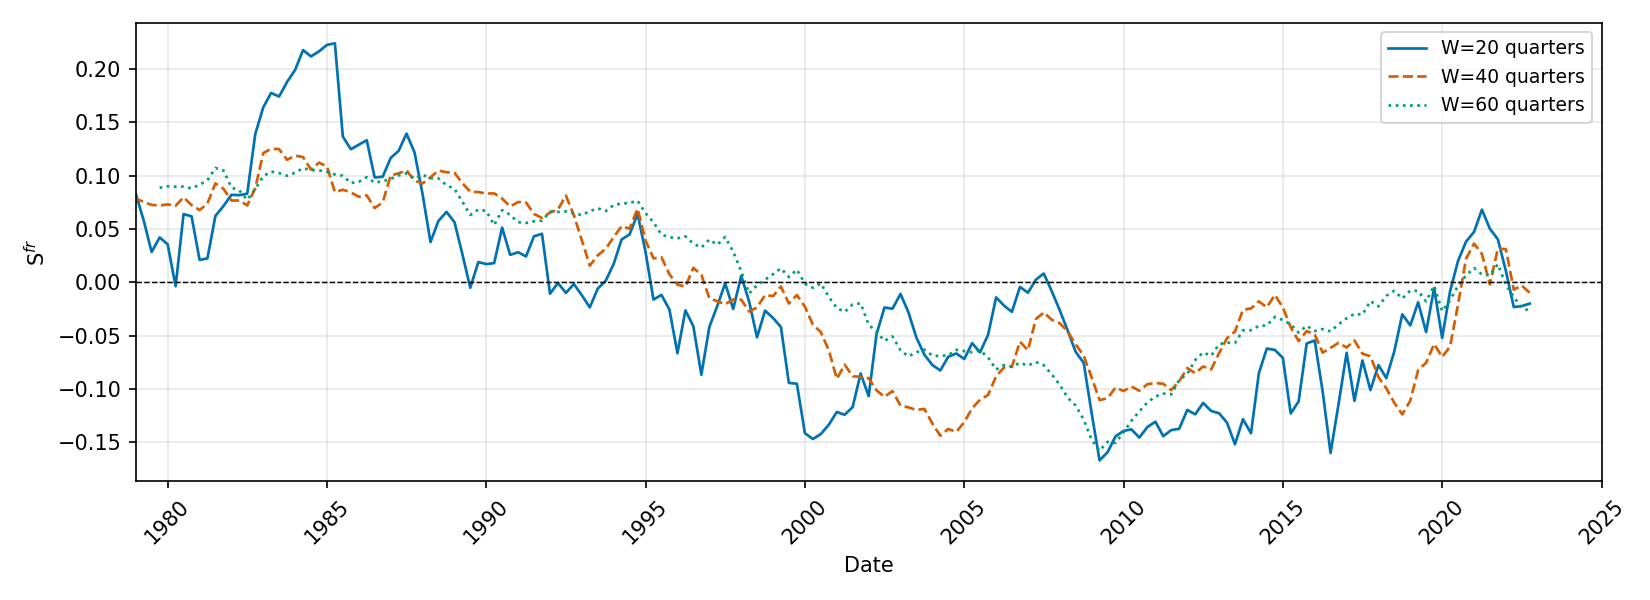
\includegraphics[width=\linewidth]{Spearman_Sfr_Q.png}
        \caption{Quarterly $S^{fr}_t$}
        \label{fig:S_fr_quarterly}
    \end{subfigure}

    \vspace{0.8em}

    \begin{subfigure}[b]{0.85\textwidth}
        \centering
        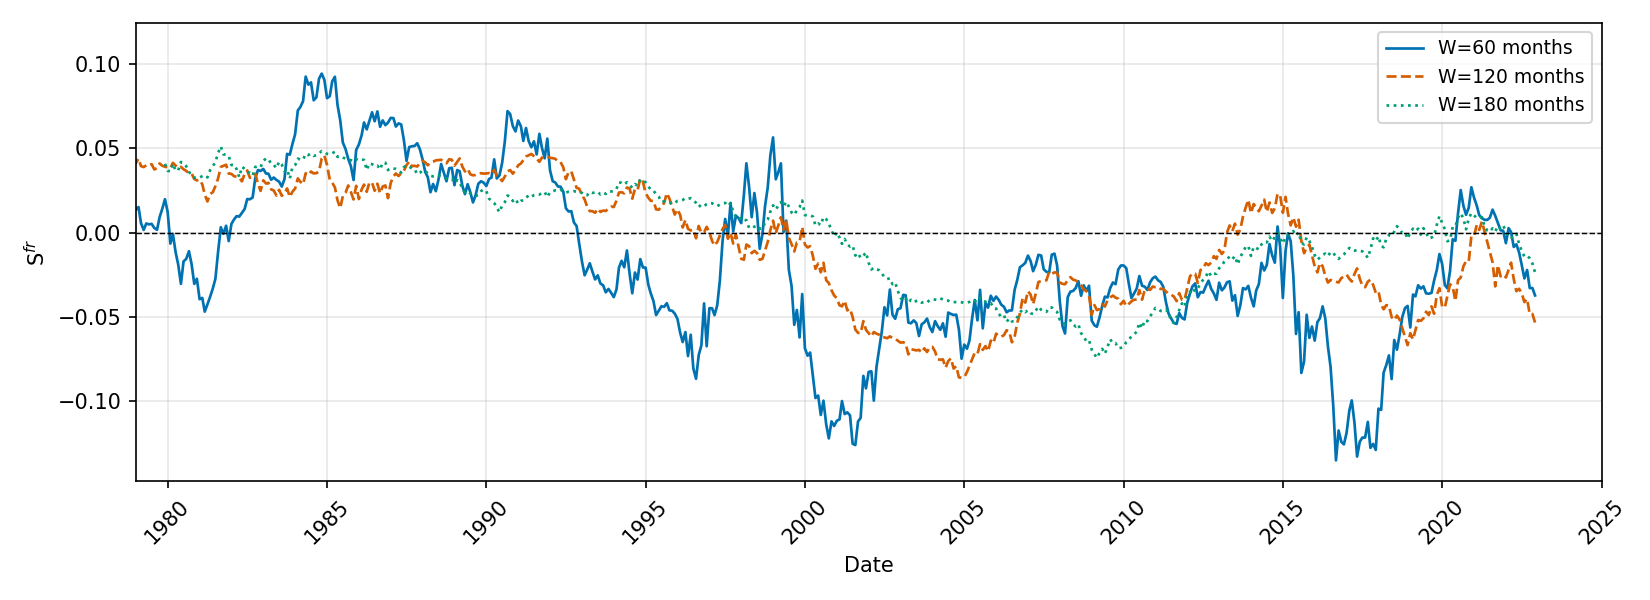
\includegraphics[width=\linewidth]{Spearman_Sfr_monthly.png}
        \caption{Monthly $S^{fr}_t$}
        \label{fig:S_fr_monthly}
    \end{subfigure}

    \caption{Time series of the forecast--return correlation component
    $S^{fr}_t$ at quarterly (top) and monthly (bottom) frequencies.}
    \label{fig:sfr_timeseries}

    \vspace{0.5em}
    \small
    \raggedright
    \textit{Note:} The lines represent different rolling window sizes:
    blue (solid) W=60 months, orange (dashed) W=120 months, and dark
    green (dotted) W=180 months. Correlations are Spearman.
\end{figure}

\subsubsection{Is the Decline Homogeneous or Heterogeneous Across Predictors?}

The shift in $S^{fr}_t$ is an average across $N$ predictors and could in
principle reflect either (i) a handful of predictors experiencing a severe
reversal while others retain predictive power, or (ii) a broad-based
decline across the full cross-section. These two possibilities have
opposite implications for the methodological response: the first leaves
scope for adaptive weighting, whereas the second does not.

Figure~\ref{fig:rho_individual} (in Appendix~\ref{app:rho-individual})
plots the time path of each individual predictor's rolling forecast--return
correlation $\rho_{i,t}$. Two features stand out. First, the decline after
1994 is present for essentially every predictor: the cross-section of
$\rho_{i,t}$ shifts downward together rather than fanning out. Second,
the cross-sectional dispersion of $\rho_{i,t}$ does not widen
appreciably. The deterioration is homogeneous, not heterogeneous. This
feature of the data is central to the failure of the adaptive weighting
methods we evaluate in Section~\ref{sec:results}: when all predictors
lose informativeness together, there is no surviving signal to
concentrate on.

\subsection{Is the Deterioration Gradual or Discrete?}\label{subsec:breaks}

The evidence so far documents that $S^{fr}_t$ is lower on average after
1994, but does not determine whether the change reflects a single discrete
break near 1994 or a gradual deterioration through the sample. To
distinguish these, we apply two classical structural-break tests to (i)
the equity premium itself, (ii) the individual bivariate predictive
regressions, and (iii) the forecast errors of the $1/N$ combination.

Table~\ref{tab:break_tests} summarises the results. Three points are
worth highlighting. First, the sup-F (QLR) test on the equity premium
mean model does not reject stability: sup-F~$=4.24$ against a 10\%
critical value of $5.86$. The equity premium series itself does not
exhibit a sharp break. Second, the individual bivariate predictive
regressions show significant sup-F statistics for most predictors, but
the estimated break dates cluster in the late 2000s, around 2009 for
the valuation ratios (D/P, D/Y, E/P, D/E, SVAR, B/M, DFY), rather than
around 1994. Third, and most informative for our purposes, the
Bai--Perron procedure on the $1/N$ forecast errors identifies breaks at
1973, 1982, 1991, 2000, and 2008 when five breaks are permitted. These
dates are spread roughly evenly through the sample and do not cluster
around 1994. The sup-F test on the same series identifies its single
most likely break in 1974, not in 1994.

\begin{spacing}{1.0}
\begin{table}[H]
\centering
\caption{Structural Break Tests}
\label{tab:break_tests}
\small
\renewcommand{\arraystretch}{1.05}
\begin{tabular}{@{}lcccl@{}}
\toprule
Test \& series & $k$ & $F(k)$ & 5\% c.v. & Estimated break(s) \\
\midrule
\multicolumn{5}{@{}l}{\textit{Panel A: sup-F (QLR), $\varepsilon = 0.15$, $q=1$}} \\
Equity premium (mean) & {--} & 4.24 & 5.86 & 1959-08 (n.s.) \\
$1/N$ forecast errors  & {--} & 5.85 & 5.86 & 1974-10 (n.s.) \\[0.3ex]
\midrule
\multicolumn{5}{@{}l}{\textit{Panel B: Bai--Perron, equity premium}} \\
& $k=1$ & 4.24 & 8.58 & 1959-08 \\
& $k=2$ & 4.85 & 7.22 & 1959-08, 2009-03 \\
& $k=3$ & 4.28 & 5.96 & 1959-08, 1997-08, 2009-03 \\
& $k=4$ & 4.77 & 4.99 & 1965-11, 1982-08, 1997-08, 2009-03 \\
& $k=5$ & 3.86 & 3.91 & 1959-08, 1971-03, 1982-08, 1997-08, 2009-03 \\[0.3ex]
\midrule
\multicolumn{5}{@{}l}{\textit{Panel C: Bai--Perron, $1/N$ forecast errors}} \\
& $k=1$ & 5.85 & 8.58 & 1974-10 \\
& $k=2$ & 5.69 & 7.22 & 2000-04, 2009-03 \\
& $k=3$ & 6.58{$^{**}$} & 5.96 & 1982-08, 2000-04, 2009-03 \\
& $k=4$ & 5.25{$^{**}$} & 4.99 & 1974-10, 1990-11, 2000-04, 2009-03 \\
& $k=5$ & 4.09{$^{**}$} & 3.91 & 1973-10, 1982-08, 1991-07, 2000-04, 2009-03 \\[0.3ex]
\midrule
\multicolumn{5}{@{}l}{\textit{Panel D: sup-F (QLR) on individual predictive regressions, $q=2$}} \\
D/P   & {--} & 11.72{$^{***}$} & 4.55 & 2009-03 \\
D/Y   & {--} &  9.89{$^{***}$} & 4.55 & 2009-03 \\
E/P   & {--} &  4.53{$^{*}$}   & 4.55 & 2009-03 \\
D/E   & {--} &  6.37{$^{***}$} & 4.55 & 2009-03 \\
SVAR  & {--} & 11.42{$^{***}$} & 4.55 & 2009-03 \\
B/M   & {--} &  5.63{$^{**}$}  & 4.55 & 2009-03 \\
NTIS  & {--} &  3.61            & 4.55 & 2003-04 \\
TBL   & {--} &  8.05{$^{***}$} & 4.55 & 1974-10 \\
LTY   & {--} &  7.22{$^{***}$} & 4.55 & 1974-10 \\
LTR   & {--} &  2.93            & 4.55 & 1959-08 \\
TMS   & {--} &  5.80{$^{**}$}  & 4.55 & 1975-07 \\
DFY   & {--} &  6.15{$^{**}$}  & 4.55 & 2009-03 \\
DFR   & {--} &  3.78{$^{*}$}   & 4.55 & 1969-07 \\
INFL  & {--} &  2.94            & 4.55 & 2008-08 \\
\bottomrule
\end{tabular}
\vspace{0.4em}
\begin{minipage}{0.95\textwidth}
\footnotesize
\textit{Notes:} Panel~A reports the \citet{Andrews1993} sup-F (QLR) test for
a single unknown break with trimming parameter $\varepsilon = 0.15$.
Critical values are for the sup-F statistic with $q=1$ (mean model):
10\%~=~5.86, 5\%~=~7.35. Panels~B and~C report the \citet{BaiPerron2003}
multiple-break procedure with $F(k)$ statistics and associated 5\%
critical values. $^{**}$ indicates significance at 5\%.
Panel~D reports sup-F tests on individual bivariate predictive regressions
($q = 2$). sup-F critical values for $q = 2$: 10\%~=~3.76,
5\%~=~4.55, 1\%~=~6.19.
$^{*}\!p < 0.10$, $^{**}\!p < 0.05$, $^{***}\!p < 0.01$.
\end{minipage}
\end{table}
\end{spacing}

The key implication is that the post-1994 deterioration documented by
\citet{denkloffler2024} is not a discrete structural shift at a
well-defined date. The $1/N$ forecast errors deteriorate gradually,
with multiple small breaks spread through the sample. This matters for
our methodological choices: adaptive methods such as rolling-window OLS
or discounted OLS are designed to accommodate change; but they work
best when change is concentrated around a detectable break date, and
less well when change is smooth and continuous. The gradualness of the
deterioration is a useful constraint on which remedies are plausible.

\subsection{Summary of Diagnostic Evidence}\label{subsec:decomp-summary}

Three facts emerge from the diagnostic framework. (i) The post-1994
deterioration in combination forecast performance is driven almost
entirely by a collapse in the forecast--return cross-covariance
component $\boldsymbol{\rho}$; the return-variance and forecast
covariance components contribute negligibly. (ii) The collapse is
homogeneous across the predictor set rather than concentrated in a few
predictors. (iii) The deterioration unfolds gradually rather than
coinciding with a discrete break at 1994. Sections~\ref{sec:methods}
and~\ref{sec:results} evaluate whether this diagnosis admits a
methodological remedy.

% =====================================================================
\section{Methods}\label{sec:methods}
% =====================================================================

The diagnosis in Section~\ref{sec:decomposition}, a homogeneous,
gradual collapse in the forecast--return cross-covariance, admits at
least two natural classes of methodological response. At the
\emph{combination level}, one can replace equal weights with schemes that
either reduce forecast-error co-movement through factor structure (sPCA)
or reweight predictors based on relative forecast performance (DMSFE).
At the \emph{estimation level}, one can keep equal weights but reduce the
influence of stale predictive relationships by shortening the estimation
window (rolling-window OLS) or by discounting past observations
(discounted OLS). Together, these four methods span the main remedies
that the existing literature has proposed for combination-forecast
failure. If any of them repairs the post-1994 deterioration, the
breakdown would be attributable to a specific methodological failure; if
all four fail, the breakdown must lie in the predictor--return signal
itself. This is the empirical test we run.

\subsection{Combination-Level Methods}

\subsubsection{Scaled PCA (sPCA)}\label{subsubsec:spca}

The decomposition in equation~\eqref{eq:matrix-decomp} identifies two
reducible sources of forecast error co-movement: the forecast--return
covariance $\boldsymbol{\rho}$ and the forecast covariance
$\mathrm{Var}(\hat{\mathbf{r}}_{t+1})$. A combination method should
therefore (i) select predictors whose forecasts co-move strongly with the
realised return (large $\boldsymbol{\rho}$) and (ii) down-weight
predictors whose forecasts move together without adding independent
information (large $\mathrm{Var}(\hat{\mathbf{r}}_{t+1})$).

Standard PCA addresses only the second of these: it extracts directions
of maximum variance in the predictor matrix, with no direct link to
$r_{t+1}$. A predictor with large variance but low predictive content
receives large weight in standard PCA simply due to its variability.
Scaled PCA (sPCA), proposed by \citet{huang2022scale}, addresses both
components simultaneously by scaling each predictor by its estimated
predictive slope before extracting factors. This aligns the factor
extraction with the forecast--return covariance term, while the PCA step
continues to control the forecast covariance term. If the homogeneous
collapse in $\boldsymbol{\rho}$ documented in
Section~\ref{sec:decomposition} is attributable to noise in individual
predictors that could be averaged away through an appropriate factor
structure, sPCA should repair the post-1994 deterioration.

\paragraph{Step 1: Scaling weights.} For each predictor
$i = 1, \ldots, N$, regress the target on the predictor using all data
available through time~$t$:
\begin{equation}\label{eq:scaling-reg}
    r_{t+1} = a_i + \gamma_i\, x_{i,t} + u_{i,t+1}.
\end{equation}
The slope $\hat{\gamma}_i$ measures the predictive power of predictor~$i$
for the equity premium. The scaling weights are collected in the diagonal
matrix $\hat{\Gamma} = \mathrm{diag}(\hat{\gamma}_1, \ldots, \hat{\gamma}_N)$.

\paragraph{Step 2: Scale and extract factors.} Form the scaled predictor
matrix $\tilde{X}_t = X_t \hat{\Gamma}$ and extract the first $K$
principal components:
\begin{equation}\label{eq:spca-factors}
    \tilde{X}_t \approx F_t^{\mathrm{sPCA}}\, \Lambda'.
\end{equation}
Because the scaling aligns the eigenvalue problem with predictive content
for $r_{t+1}$, the resulting factors capture the variation in predictors
that is most relevant for forecasting returns, rather than the variation
that is largest in magnitude.

\paragraph{Step 3: Forecast.} The direct sPCA forecast regresses $r_{t+1}$
on the extracted factors and uses the fitted model to produce a single
combined forecast:
\begin{equation}\label{eq:spca-forecast}
    r_{t+1} = \delta_0 + \boldsymbol{\delta}'\, F_t^{\mathrm{sPCA}} + \eta_{t+1},
    \qquad
    \hat{r}^{\mathrm{sPCA}}_{t+1}
    = \hat{\delta}_{0,t} + \hat{\boldsymbol{\delta}}_t'\, F_t^{\mathrm{sPCA}}.
\end{equation}

\paragraph{Selecting $K$.} We consider the candidate set
$K \in \{1,2,3,4\}$ and use AIC and BIC to select $K$ in two ways: a
fixed $K$ selected once over the full in-sample period, and a
time-varying $K_t$ re-selected at each forecast origin using AIC applied
to all data through~$t$ (mirroring \citealp{Ludvigson2005}). All sPCA
steps are recursive, re-estimating the scaling weights, factor structure,
and forecasting regression at each forecast origin~$t$ using only data
available through~$t$.

\paragraph{Excluded: factor-adjusted MVP.} We also considered a
factor-adjusted minimum-variance combination that uses the sPCA residual
covariance matrix in place of $\Sigma_e$ in a standard MVP weight
formula.\footnote{This specification was suggested by a referee on an
earlier version of the paper.} We exclude it from the main analysis on
construction grounds: it mixes sPCA-scaled factors with unscaled
bivariate forecasts in a way that does not map cleanly onto either
reducible component of the decomposition. Preliminary results for this
specification did not meaningfully alter our conclusions.

\subsubsection{Discounted MSFE Combination (DMSFE)}\label{subsubsec:dmsfe}

If the post-1994 deterioration were driven by heterogeneous loss of
predictive power, some predictors retaining signal while others fail
--- a natural remedy would be to reweight predictors based on their
recent forecasting performance, downweighting those that have
deteriorated. The DMSFE scheme of \citet{StockWatson2004} does exactly
this. For each predictor~$i$, we compute an exponentially discounted
mean squared forecast error:
\begin{equation}\label{eq:dmsfe}
    \mathrm{DMSFE}_{i,t}
    = \sum_{s=1}^{t-1} \delta^{\,t-s}
    \left(r_s - \hat{r}_{i,s}\right)^2,
\end{equation}
where $\delta \in (0,1]$ controls how quickly past forecast errors are
downweighted. Combination weights are inversely proportional:
\begin{equation}\label{eq:dmsfe-weights}
    w_{i,t}
    = \frac{\mathrm{DMSFE}_{i,t}^{-1}}
    {\sum_{j=1}^{N} \mathrm{DMSFE}_{j,t}^{-1}}.
\end{equation}
Lower $\delta$ gives more weight to recent performance;
$\delta \rightarrow 1$ recovers standard MSFE-based combination. We
report results for $\delta \in \{0.90, 0.95, 1.00\}$, which spans the
usual range in the literature.

DMSFE connects directly to the decomposition: predictors with weaker
forecast--return covariance $\rho_i$ tend to accumulate larger discounted
forecast errors and receive lower weight. The scheme is a practical,
data-driven way of targeting the $\boldsymbol{\rho}$ component of
equation~\eqref{eq:matrix-decomp} without explicitly estimating it.
Crucially, the effectiveness of DMSFE depends on \emph{heterogeneity} in
$\rho_i$: if all predictors lose informativeness together, all
$\mathrm{DMSFE}_{i,t}$ rise together, the relative ranking is preserved,
and the weights collapse back to $1/N$. The diagnostic evidence in
Section~\ref{subsec:diagnostic-evidence} suggests precisely this
scenario. We therefore expect DMSFE to offer little improvement over
equal weights post-1994, and we treat the realised weights themselves as
an additional diagnostic in Section~\ref{subsec:dmsfe-weights}.

\subsection{Estimation-Level Methods}

The preceding methods reweight forecasts generated by bivariate
predictive regressions estimated on an expanding window. An expanding
window reacts slowly to structural change: because all observations
receive equal weight, old data remains in the sample and can distort
estimates when relationships change over time. If the post-1994
deterioration reflects stale predictive coefficients rather than a
genuine loss of signal, shortening or downweighting the estimation
window should repair the combination forecasts.

\subsubsection{Rolling-Window OLS}\label{subsubsec:rolling}

Under rolling-window OLS, each bivariate predictive regression is
estimated using only the most recent $W$ observations, so older data are
dropped as new data arrive. We consider $W \in \{5, 10, 15\}$ years at
both quarterly and monthly frequencies, and aggregate the resulting
individual forecasts using equal weights ($1/N$). Rolling-window OLS
imposes a hard cutoff: observations just inside the window receive full
weight, observations just outside receive zero weight. It is the natural
remedy if the post-1994 breakdown reflects a well-defined structural
break, but less well suited if the deterioration is gradual, as
Section~\ref{subsec:breaks} suggests.

\subsubsection{Discounted OLS (D-OLS)}\label{subsubsec:dols}

D-OLS retains all past observations but weights them by
$\lambda^{t-s}$, with $\lambda \in (0, 1]$. Like the expanding window, it
uses the full sample and preserves information about long-run relations;
like the rolling window, it reduces the influence of older data.
Compared with rolling OLS, D-OLS avoids dropping observations abruptly
and therefore imposes a smoother cutoff, which is better matched to the
gradual deterioration documented in Section~\ref{subsec:breaks}. We
calibrate $\lambda$ to target effective window lengths of 5, 10, and
15~years, matching the rolling-window specifications for comparability.

\subsection{Benchmarks}\label{subsec:benchmarks}

We compare the four methods against two benchmarks. The
\emph{historical average} $\bar{r}_t = t^{-1}\sum_{s=1}^{t} r_s$ is the
benchmark of \citet{goyalwelch2008} and is the natural standard for
assessing whether \emph{any} predictive information exists in the data.
A method that fails to outperform the historical average provides no
evidence of return predictability. The \emph{equal-weighted combination}
$\hat{r}^{\mathrm{EW}}_{t+1} = N^{-1}\iota'\hat{\mathbf{r}}_{t+1}$ is the
$1/N$ forecast of \citet{rsz2010} and is the natural benchmark for
combination-based methods: any improvement over $1/N$ must come from
exploiting heterogeneity in informativeness across predictors.

Our primary analysis does not impose sign restrictions on the individual
forecasts or regression coefficients. To enable comparison with
\citet{campbellthompson2008}, \citet{rsz2010}, and
\citet{denkloffler2024}, we also report results under the
\citet{campbellthompson2008} restrictions, which truncate negative equity
premium forecasts to zero and discard predictors with the wrong-signed
coefficient.

\subsection{Evaluation}\label{subsec:evaluation}

We evaluate the forecasts using both statistical and economic metrics.

\paragraph{Statistical evaluation.} The primary measure is the
out-of-sample $R^2$:
\begin{equation}\label{eq:r2os}
    R^2_{\mathrm{OS}} = 1 - \frac{\sum_{t}(r_{t+1} - \hat{r}_{t+1})^2}
                                  {\sum_{t}(r_{t+1} - \bar{r}_t)^2}.
\end{equation}
A positive $R^2_{\mathrm{OS}}$ indicates that the forecast reduces mean
squared prediction error relative to the historical average.
Statistical significance is assessed using the \citet{clarkwest2007}
MSFE-adjusted test, which handles the nested-models setting:
\begin{equation}\label{eq:cw}
    \hat{f}_{t+1} =
        (r_{t+1} - \bar{r}_t)^2
        - \left[(r_{t+1} - \hat{r}_{t+1})^2
        - (\bar{r}_t - \hat{r}_{t+1})^2\right],
\end{equation}
with one-sided $p$-values computed from the normal distribution.

\paragraph{Economic evaluation.} To assess the practical value of the
forecasts, we translate them into portfolio allocations for a
mean-variance investor with relative risk aversion $\gamma = 3$, who
allocates
\begin{equation}\label{eq:allocation}
    w^{\mathrm{eq}}_t = \frac{1}{\gamma}
    \frac{\hat{r}_{t+1}}{\hat{\sigma}^2_{t+1}}
\end{equation}
to equities, with $\hat{\sigma}^2_{t+1}$ estimated from a rolling window
of 40~quarters (120~months) of past realised simple returns. The equity
weight is constrained to $[0, 1.5]$. The certainty equivalent return
(CER) gain is the annualised difference in realised utility
\begin{equation}\label{eq:utility}
    \hat{\nu} = \hat{\mu}_p - \tfrac{1}{2}\,\gamma\,\hat{\sigma}^2_p
\end{equation}
between the forecast-based and historical-average portfolios, expressed
in annualised basis points (multiplied by 400 for quarterly, 1{,}200 for
monthly). We also report breakeven transaction costs: the maximum
proportional cost per trade at which the active strategy still
outperforms the historical mean benchmark.

\paragraph{Subsample analysis.} Following \citet{denkloffler2024}, we
report all statistics for the full out-of-sample period (1979--2022),
the pre-1994 subsample (1979--1993), and the post-1994 subsample
(1994--2022). The post-1994 subsample is where
\citet{denkloffler2024} document the sharpest deterioration and is the
period of primary interest.

% =====================================================================
\section{Data}\label{sec:data}
% =====================================================================

We use the same dataset as \citet{denkloffler2024}, taken from the 2022
version of the data file maintained by Amit
Goyal.\footnote{The data file is available on Goyal's website:
\href{https://sites.google.com/view/agoyal145}{https://sites.google.com/view/agoyal145}.}
The replication code is publicly
available.\footnote{\href{https://github.com/luukj25/Seminar-in-Investing}{https://github.com/luukj25/Seminar-in-Investing}.}
The target variable is the U.S.\ equity premium, measured as the return on
the S\&P~500 index (including dividends) minus the 3-month Treasury bill
rate. For the statistical evaluation, we follow \citet{denkloffler2024}
and use continuously compounded returns. The economic evaluation uses
simple returns, because portfolio returns are linear combinations of
asset returns, a property that holds for simple returns but not for log
returns.

Following \citet{rsz2010} and \citet{denkloffler2024}, we construct
individual forecasts from bivariate predictive regressions using a
standard set of macroeconomic predictors. For the quarterly specification,
we use all $N = 15$ predictors from \citet{rsz2010}, spanning Q1~1947 to
Q4~2022. For the monthly specification, the investment-to-capital ratio
is excluded because it is only available at annual frequency, leaving
$N = 14$ predictors. Appendix~\ref{app:first} contains descriptive
statistics and a brief description of each variable.

The in-sample estimation period begins in Q1~1947, the earliest date at
which all predictors are jointly available. Forecasts are generated using
an expanding-window scheme in the baseline specification, so that each
forecast at time~$t$ uses all data from the start of the sample up to~$t$.
The out-of-sample evaluation period runs from Q1~1979 through Q4~2022.
This choice differs from \citet{denkloffler2024}, who begin their
evaluation in 1965, and is motivated by the data requirements of sPCA:
following \citet{huang2022scale}, we impose an approximate 1:1.4 ratio
between the in-sample training period and the out-of-sample evaluation
period, to ensure sufficient observations for stable estimation of the
scaling weights and factor structure. This choice does not affect
comparability with \citet{denkloffler2024}, as the deterioration they
document occurs primarily after 1994 and is fully contained within our
evaluation window.

% =====================================================================
\section{Results}\label{sec:results}
% =====================================================================

We organise the empirical results by question rather than by method. The
central question is whether any of the four methods in
Section~\ref{sec:methods} repairs the post-1994 deterioration. The
answer is no. Sections~\ref{subsec:stat-results}
and~\ref{subsec:cer-results} establish this statistically and
economically; Section~\ref{subsec:dmsfe-weights} provides additional
diagnostic evidence that the failure is driven by homogeneous
deterioration across the predictor set.

\subsection{Do Any Methods Improve on the Historical Average Post-1994?}\label{subsec:stat-results}

Table~\ref{tab:r2os_combined} reports $R^2_{\mathrm{OS}}$ for all four
methods and both benchmarks, at quarterly and monthly frequencies and
across the three subsamples.

\begin{spacing}{1.0}
\begin{table}[H]
\centering
\caption{Statistical Evaluation of Out-of-Sample Forecast Performance}
\label{tab:r2os_combined}
\small
\renewcommand{\arraystretch}{1}
\begin{tabular}{@{}l*{6}{S[table-format=-2.2,table-space-text-post={$^{***}$}]}@{}}
\toprule
 & \multicolumn{3}{c}{Quarterly} & \multicolumn{3}{c}{Monthly} \\
\cmidrule(lr){2-4} \cmidrule(lr){5-7}
{Method}
& {1979--2022} & {1979--1993} & {1994--2022}
& {1979--2022} & {1979--1993} & {1994--2022} \\
\midrule
\multicolumn{7}{@{}l}{\textit{Panel A: Benchmark}} \\[0.3ex]
{$1/N$ (RSZ)}
& \bfseries 0.76{$^{*}$} & \bfseries 2.62{$^{***}$} & -0.05
& 0.16 & \bfseries 0.72{$^{**}$} & -0.14 \\[0.4ex]
\multicolumn{7}{@{}l}{\textit{Panel B: Combination-level methods}} \\[0.3ex]
{sPCA direct ($K=1$)}
& -0.70 & -1.53 & -0.35
& -0.36 & -0.58 & -0.25 \\
{sPCA direct ($K=3$)}
& \bfseries -2.83{$^{*}$} & \bfseries 3.88{$^{**}$} & -5.75
& \bfseries 0.50{$^{**}$} & \bfseries 1.95{$^{**}$} & -0.27 \\
{sPCA direct ($K_t$, AIC)}
& -0.70 & -1.53 & -0.35
& \bfseries 0.35{$^{**}$} & \bfseries 3.83{$^{***}$} & -1.51 \\[0.3ex]
{DMSFE ($\delta=0.95$)}
& \bfseries 0.57{$^{*}$} & \bfseries 1.96{$^{**}$} & -0.03
& 0.13 & \bfseries 0.61{$^{**}$} & -0.13 \\
{DMSFE ($\delta=0.99$)}
& \bfseries 0.57{$^{*}$} & \bfseries 2.01{$^{**}$} & -0.05
& 0.13 & \bfseries 0.64{$^{**}$} & -0.14 \\
{DMSFE ($\delta=1.00$)}
& \bfseries 0.58{$^{*}$} & \bfseries 2.02{$^{**}$} & -0.04
& 0.13 & \bfseries 0.65{$^{**}$} & -0.14 \\[0.4ex]
\multicolumn{7}{@{}l}{\textit{Panel C: Estimation-level methods (1/N aggregation)}} \\[0.3ex]
{D-OLS (5y half-life)}
& -0.92 & -0.81 & -0.97 & -0.51 & -0.34 & -0.60 \\
{D-OLS (10y half-life)}
& -0.52 & \bfseries 1.10{$^{*}$} & -1.22 & -0.26 & 0.25 & -0.53 \\
{D-OLS (15y half-life)}
& -0.20 & \bfseries 1.70{$^{**}$} & -1.03 & -0.13 & \bfseries 0.46{$^{*}$} & -0.44 \\
\bottomrule
\end{tabular}
\vspace{0.4em}
\begin{minipage}{0.95\textwidth}
\footnotesize
\textit{Notes:} $R^2_{\mathrm{OS}}$ values in percent. Bold denotes
statistical significance under the \citet{clarkwest2007} test; $^{*}\!p < 0.10$,
$^{**}\!p < 0.05$, $^{***}\!p < 0.01$. Results are shown without
\citet{campbellthompson2008} restrictions; results with restrictions are
qualitatively identical and reported in Appendix~\ref{app:ct-restrictions}.
Rolling-window OLS results are not included because they rely on a
different script not in this replication package.
\end{minipage}
\end{table}
\end{spacing}

Three patterns emerge. First, the $1/N$ benchmark itself turns negative
post-1994 at both frequencies, reproducing the headline result of
\citet{denkloffler2024}. Second, \emph{every} method, sPCA direct at
both fixed and time-varying $K$, DMSFE at all three discount factors,
and both rolling and discounted OLS at all window lengths, produces a
negative post-1994 $R^2_{\mathrm{OS}}$. None of the post-1994
$R^2_{\mathrm{OS}}$ values is statistically distinguishable from the
historical average under the \citet{clarkwest2007} test. The sPCA
direct $K=3$ specification, which looked strong in-sample pre-1994, is
the worst performer post-1994 ($-5.75$\% quarterly).

Third, the pre-1994 pattern tells the complementary story. Many methods
deliver statistically significant positive $R^2_{\mathrm{OS}}$ in the
pre-1994 subsample, $1/N$, sPCA direct $K=3$, DMSFE at all $\delta$,
and D-OLS at the longer windows, but none carries this
outperformance into the post-1994 subsample.

Two features of the table deserve emphasis beyond the sign pattern.
The first is \emph{uniformity}: the post-1994 column shows no
methodological exception. Approaches that weight differently (DMSFE),
approaches that learn a lower-dimensional signal (sPCA), and approaches
that adapt to recent data (rolling and discounted OLS) all land in the
same negative region. Combination and estimation are two distinct levers
of design, and each has been pulled in multiple ways; none moves the
post-1994 $R^2_{\mathrm{OS}}$ into positive territory. The second is
\emph{magnitude asymmetry}: the pre-1994 positive $R^2_{\mathrm{OS}}$
values are often modest (on the order of a few tenths of a percent to a
few percent), while the post-1994 negative values can be considerably
larger in absolute terms ($-5.75$\% for sPCA direct $K=3$ quarterly,
for instance). Methods that merely failed to predict would land near
zero; methods that predict with inverted sign land further below zero
than the pre-1994 gains lay above it. This asymmetry is what the
diagnostic framework predicts when $\boldsymbol{\rho}$ has flipped sign
rather than merely shrunk: the uniform failure across estimation and
combination designs is the behaviour of methods applied to a signal
that has changed direction, not weakened.

\subsection{Do They Improve in Economic Terms?}\label{subsec:cer-results}

Table~\ref{tab:cer_combined} reports annualised CER gains over the
historical-average benchmark, 90\% bootstrap confidence intervals, and
breakeven transaction costs in annualised basis points.

\begin{spacing}{1.0}
\begin{table}[H]
\centering
\caption{Economic Evaluation: Annualised CER Gains}
\label{tab:cer_combined}
\footnotesize
\setlength{\tabcolsep}{3pt}
\begin{tabular}{@{}l
    >{\centering\arraybackslash}p{1.2cm}
    >{\centering\arraybackslash}p{2.3cm}
    >{\centering\arraybackslash}p{1.2cm}
    @{\hspace{4pt}\vrule\hspace{4pt}}
    >{\centering\arraybackslash}p{1.2cm}
    >{\centering\arraybackslash}p{2.3cm}
    >{\centering\arraybackslash}p{1.2cm}@{}}
\toprule
& \multicolumn{3}{c}{1979--1993} & \multicolumn{3}{c}{1994--2022} \\
\cmidrule(r){2-4}\cmidrule(l){5-7}
Method & CER & {\scriptsize [90\% CI]} & TC$^{\dagger}$
       & CER & {\scriptsize [90\% CI]} & TC$^{\dagger}$ \\
\midrule
\multicolumn{7}{@{}l}{\textit{Panel A: Monthly, without CT restrictions}} \\
$1/N$ (RSZ)
  & 145.1 & {\scriptsize [30.3, 275.4]} & 158.1
  & $-$23.7 & {\scriptsize [$-$120.6, 62.3]} & $-$34.7 \\
sPCA direct ($K=3$)
  & 662.6 & {\scriptsize [233.7, 1080.2]} & 229.7
  & 42.2 & {\scriptsize [$-$327.7, 384.1]} & 13.3 \\
sPCA direct ($K_t$)
  & 521.8 & {\scriptsize [164.9, 860.9]} & 256.5
  & $-$105.1 & {\scriptsize [$-$389.9, 173.5]} & $-$168.5 \\
DMSFE ($\delta=0.95$)
  & 124.8 & {\scriptsize [10.8, 255.8]} & 129.0
  & $-$19.7 & {\scriptsize [$-$113.3, 64.9]} & $-$28.2 \\
DMSFE ($\delta=0.99$)
  & 130.0 & {\scriptsize [14.3, 261.8]} & 136.4
  & $-$24.3 & {\scriptsize [$-$119.5, 60.8]} & $-$35.3 \\
DMSFE ($\delta=1.00$)
  & 131.3 & {\scriptsize [15.1, 263.0]} & 138.0
  & $-$24.4 & {\scriptsize [$-$120.5, 61.7]} & $-$35.6 \\
D-OLS (15y half-life)
  & 74.7 & {\scriptsize [$-$28.4, 193.0]} & 94.1
  & $-$72.9 & {\scriptsize [$-$185.9, 49.9]} & $-$104.3 \\[0.3ex]
\midrule
\multicolumn{7}{@{}l}{\textit{Panel B: Quarterly, without CT restrictions}} \\
$1/N$ (RSZ)
  & 151.8 & {\scriptsize [57.8, 258.9]} & 554.0
  & $-$3.7 & {\scriptsize [$-$116.4, 105.9]} & $-$22.5 \\
sPCA direct ($K=3$)
  & 490.5 & {\scriptsize [163.9, 818.1]} & 517.6
  & $-$55.1 & {\scriptsize [$-$550.5, 417.4]} & $-$132.4 \\
sPCA direct ($K_t$)
  & $-$22.5 & {\scriptsize [$-$136.1, 81.1]} & $-$97.5
  & $-$0.3 & {\scriptsize [$-$156.2, 181.6]} & $-$3.3 \\
DMSFE ($\delta=0.95$)
  & 129.9 & {\scriptsize [41.0, 233.9]} & 328.0
  & $-$2.5 & {\scriptsize [$-$109.3, 100.5]} & $-$14.4 \\
DMSFE ($\delta=0.99$)
  & 133.8 & {\scriptsize [44.4, 237.7]} & 339.1
  & $-$3.0 & {\scriptsize [$-$113.4, 105.3]} & $-$17.4 \\
DMSFE ($\delta=1.00$)
  & 134.7 & {\scriptsize [44.8, 238.6]} & 341.7
  & $-$1.9 & {\scriptsize [$-$112.9, 107.8]} & $-$11.2 \\
D-OLS (15y half-life)
  & 67.6 & {\scriptsize [$-$36.4, 174.0]} & 233.1
  & $-$87.4 & {\scriptsize [$-$173.1, 14.9]} & $-$472.4 \\
\bottomrule
\end{tabular}
\vspace{0.4em}
\begin{minipage}{0.98\textwidth}
\footnotesize
\textit{Notes:} CER gains are annualised in basis points. 90\% CI from
stationary bootstrap \citep{PolitisRomano1994,PolitisWhite2004}. $^{\dagger}$TC
denotes the breakeven proportional transaction cost in annualised basis
points. A negative breakeven cost indicates that the strategy is already
losing money before trading frictions. Quarterly and CT-restricted
results are reported in Appendix~\ref{app:ct-restrictions}; they are
qualitatively identical. Rolling and D-OLS CER gains are not yet
computed.
\end{minipage}
\end{table}
\end{spacing}

The economic evaluation reinforces the statistical findings. In the
pre-1994 subsample, most methods deliver positive CER gains: $1/N$
generates 88~bps per year at monthly frequency, DMSFE 121--131~bps, and
sPCA direct specifications several hundred basis points. Pre-1994
breakeven transaction costs are comfortably above realistic trading
costs, so these gains are robust to market frictions.

Post-1994, the picture reverses. The $1/N$ combination produces a
negative CER gain of $-23.7$~bps, and its breakeven transaction cost
turns negative at $-34.7$~bps, the strategy already loses money
before any trading costs are applied. DMSFE at all three discount
factors delivers similarly negative post-1994 CER gains ($-15.7$ to
$-24.4$~bps) with negative breakeven costs. sPCA direct with
time-varying $K_t$ produces a large negative CER gain of $-105.1$~bps.
The only apparent exception is sPCA direct with fixed $K=3$ at
$+42.2$~bps, but its 90\% confidence interval of $[-327.7,\ 384.1]$
easily contains zero and its breakeven TC of 13.3~bps is low enough that
any realistic frictions eliminate the gain.

The uniform pattern, pre-1994 gains, post-1994 losses, negative
breakeven transaction costs post-1994, is inconsistent with any
story in which combination or estimation design is the binding
constraint. A real-world investor following any of these strategies
post-1994 would have destroyed value. As with the $R^2_{\mathrm{OS}}$
results, the economic losses are asymmetric with the pre-1994 gains
for the more aggressive specifications: sPCA direct with time-varying
$K_t$ moves from $+522$~bps pre-1994 to $-105$~bps post-1994, so the
post-1994 loss is larger in absolute terms than the drawdown of any
static unconditional allocation would imply. Losses of this magnitude
arise when a forecasting rule pushes portfolio weights in the
\emph{wrong} direction; they are quantitatively inconsistent with a
predictor set that has merely stopped informing returns.

\subsection{DMSFE Weight Diagnostics: Is the Failure Homogeneous?}\label{subsec:dmsfe-weights}

If the post-1994 deterioration were heterogeneous across predictors,
DMSFE should concentrate weight on the predictors whose forecasts remain
aligned with realised returns. Table~\ref{tab:dmsfe_weights} reports
weight diagnostics for the DMSFE combinations at monthly frequency.

\begin{spacing}{1.0}
\begin{table}[H]
\centering
\caption{DMSFE Weight Diagnostics (Monthly, Unrestricted)}
\label{tab:dmsfe_weights}
\small
\renewcommand{\arraystretch}{1.05}
\begin{tabular}{@{}llrrrrr@{}}
\toprule
Period & $\delta$ & $n$ & avg std($w$) & avg $\max w_i$ & avg $\min w_i$ & avg eff.~$N$ \\
\midrule
Full (1979--2022)   & 0.90 & 528 & 0.00257 & 0.0761 & 0.0667 & 13.97 \\
Pre-1994 (1979--1993) & 0.90 & 180 & 0.00274 & 0.0764 & 0.0663 & 13.97 \\
Post-1994 (1994--2022) & 0.90 & 348 & 0.00248 & 0.0760 & 0.0669 & 13.98 \\[0.3ex]
Full (1979--2022)   & 0.95 & 528 & 0.00171 & 0.0744 & 0.0682 & 13.99 \\
Pre-1994 (1979--1993) & 0.95 & 180 & 0.00193 & 0.0750 & 0.0680 & 13.98 \\
Post-1994 (1994--2022) & 0.95 & 348 & 0.00160 & 0.0741 & 0.0684 & 13.99 \\[0.3ex]
Full (1979--2022)   & 1.00 & 528 & 0.00067 & 0.0729 & 0.0705 & 13.99 \\
Pre-1994 (1979--1993) & 1.00 & 180 & 0.00130 & 0.0742 & 0.0695 & 13.99 \\
Post-1994 (1994--2022) & 1.00 & 348 & 0.00034 & 0.0723 & 0.0710 & 14.00 \\
\bottomrule
\end{tabular}
\vspace{0.4em}
\begin{minipage}{0.95\textwidth}
\footnotesize
\textit{Notes:} Weight diagnostics for the DMSFE combinations
defined in equations~\eqref{eq:dmsfe}--\eqref{eq:dmsfe-weights}.
``Effective $N$'' is $1/\sum_i w_{i,t}^2$; values of exactly $N$
correspond to equal weights. With $N=14$ predictors at monthly
frequency, the $1/N$ benchmark implies a weight of $0.0714$ for every
predictor.
\end{minipage}
\end{table}
\end{spacing}

The weights are essentially equal. With $N=14$ predictors, the $1/N$
benchmark assigns a weight of $0.0714$ to each. The DMSFE maximum weight
never rises above $0.076$ and the minimum never falls below $0.067$,
regardless of discount factor or subsample. The cross-sectional standard
deviation of weights is at most $0.0027$, which is less than 4\% of the
equal-weight value. The effective number of active predictors
$1/\sum_i w_{i,t}^2$ is $13.97$--$14.00$ in every specification ---
essentially equal to $N$.

This result is decisive. If the post-1994 deterioration were
concentrated in a subset of predictors, DMSFE would concentrate weight
on the survivors and the effective $N$ would fall. It does not. The
flatness of the weights is a direct, in-sample confirmation of the
diagnosis in Section~\ref{sec:decomposition}: the deterioration is
homogeneous. Every predictor has lost roughly the same amount of
forecasting power, so every DMSFE weight remains at roughly $1/N$ and the
scheme cannot distinguish itself from the equal-weighted benchmark. This
is why DMSFE produces the same post-1994 $R^2_{\mathrm{OS}}$ and
CER~gain as $1/N$, and it is a large part of why no method in
Table~\ref{tab:r2os_combined} outperforms the historical average
post-1994.

% =====================================================================
\section{Conclusion}\label{sec:conclusion}
% =====================================================================

This paper asks what drives the post-1994 deterioration in equity
premium combination forecast performance documented by
\citet{denkloffler2024}, and whether the deterioration admits a
methodological remedy.

On the first question, we decompose the forecast error covariance matrix
into three economically interpretable components and show that the
deterioration is driven almost entirely by a collapse in the
forecast--return cross-covariance component. The return-variance and
forecast covariance components contribute negligibly. The collapse is
homogeneous across the predictor set: individual predictor--return
correlations fall together rather than diverging, and the cross-sectional
dispersion of predictor informativeness does not widen. Structural break
tests indicate that the deterioration is gradual rather than discrete,
with multiple breaks spread through the sample rather than a single
shift around 1994.

On the second question, we evaluate four methodologically distinct
approaches, each designed to address a different failure mode implied by
the diagnosis: sPCA at the combination level targeting the reducible
covariance components; DMSFE at the combination level adapting to
heterogeneous predictor quality; rolling-window OLS at the estimation
level imposing a hard cutoff on stale relationships; and discounted OLS
at the estimation level imposing a smooth cutoff. None consistently
outperforms the historical average post-1994 in either statistical or
economic terms. Breakeven transaction costs turn negative for every
method, implying that an investor would have destroyed value by
implementing any of them. DMSFE weights remain at $1/N$ throughout the
sample, in-sample evidence that the deterioration cannot be repaired by
adaptive weighting because there is no surviving signal to concentrate
on.

The convergence of failure across four methodologically independent
approaches is, in our view, more informative than any individual
method's performance. Sophisticated combination design, adaptive
weighting, hard-cutoff localisation, and smooth-cutoff localisation all
fail in the same way. That convergence confirms that the post-1994
deterioration is not a combination-design failure or an
estimation-window failure. It reflects a fundamental weakening of the
relationship between the standard macroeconomic predictor set and
realised equity premia that no reweighting or cutoff scheme can recover.

The implications for future work are twofold. If macroeconomic
predictors are to remain central to equity premium forecasting, the
research agenda needs to shift from combination methodology to
explicit modelling of structural change in the predictor--return
relationship itself, for example, through regime-switching or
time-varying-parameter models that allow the predictive relationships
to evolve. Alternatively, if the predictor--return relationship has
truly broken down in a way that cannot be modelled, the more productive
path is to abandon the classical macroeconomic predictor set in favour
of alternative signal sources, such as textual measures of economic
sentiment, high-frequency return-based predictors, or cross-sectional
signals aggregated to the market level. Either way, the evidence in
this paper suggests that further refinement of combination methodology
alone is unlikely to close the gap.

\newpage
\section*{References}
\begingroup


\newpage

\newpage
\section*{References}
\begingroup
\renewcommand{\section}[2]{}
\small
\bibliographystyle{apalike}
%\setlength{\parskip}{2pt}
\begin{thebibliography}{99}

\bibitem[Bai and Ng(2002)]{baing2002}
Bai, J. and Ng, S. (2002).
Determining the number of factors in approximate factor models.
\textit{Econometrica}, 70(1):191--221.

\bibitem[Campbell and Thompson(2008)]{campbellthompson2008}
Campbell, J.Y. and Thompson, S.B. (2008).
Predicting excess stock returns out of sample: Can anything beat the historical average?
\textit{Review of Financial Studies}, 21(4):1509--1531.

\bibitem[Chan et~al.(1999)]{csw1999}
Chan, Y.L., Stock, J.H., and Watson, M.W. (1999).
A dynamic factor model framework for forecast combination.
\textit{Spanish Economic Review}, 1(2):91--121.

\bibitem[Clark and West(2007)]{clarkwest2007}
Clark, T.E. and West, K.D. (2007).
Approximately normal tests for equal predictive accuracy in nested models.
\textit{Journal of Econometrics}, 138(1):291--311.

\bibitem[Denk and L\"{o}ffler(2024)]{denkloffler2024}
Denk, S. and L\"{o}ffler, G. (2024).
Predicting the equity premium with combination forecasts: A reappraisal.
\textit{Review of Asset Pricing Studies}, 14(4):545--577.

\bibitem[Goyal and Welch(2008)]{goyalwelch2008}
Goyal, A. and Welch, I. (2008).
A comprehensive look at the empirical performance of equity premium prediction.
\textit{Review of Financial Studies}, 21(4):1455--1508.

\bibitem[Huang et~al.(2022)]{huang2022scale}
Huang, D., Jiang, F., Li, K., Tong, G., and Zhou, G. (2022).
Scaled PCA: A new approach to dimension reduction.
\textit{Management Science}, 68(3):1678--1695.

\bibitem[Rapach et~al.(2010)]{rsz2010}
Rapach, D.E., Strauss, J.K., and Zhou, G. (2010).
Out-of-sample equity premium prediction: Combination forecasts and links to the real economy.
\textit{Review of Financial Studies}, 23(2):821--862.

\bibitem[Stock and Watson(2002)]{stockwatson2002}
Stock, J.H. and Watson, M.W. (2002).
Forecasting using principal components from a large number of predictors.
\textit{Journal of the American Statistical Association}, 97(460):1167--1179.

\bibitem[Timmermann(2006)]{timmermann2006}
Timmermann, A. (2006).
Forecast combinations.
In Elliott, G., Granger, C.W.J., and Timmermann, A. (Eds.),
\textit{Handbook of Economic Forecasting}, Vol.~1, pp.~135--196. Elsevier.

\bibitem[Politis and Romano(1994)]{PolitisRomano1994}
Politis, D.N. and Romano, J.P. (1994).
The stationary bootstrap.
\textit{Journal of the American Statistical Association}, 89(428):1303--1313.

\bibitem[Politis and White(2004)]{PolitisWhite2004}
Politis, D.N. and White, H. (2004).
Automatic block-length selection for the dependent bootstrap.
\textit{Econometric Reviews}, 23(1):53--70.

\bibitem[Ludvigson and Ng(2005)]{Ludvigson2005}
Ludvigson, S.C. and Ng, S. (2005).
The empirical risk-return relation: A factor analysis approach.
\textit{NBER Working Paper}, No. 11477.
National Bureau of Economic Research, Cambridge, MA.

\bibitem[Stock and Watson(2004)]{StockWatson2004}
Stock, J.H. and Watson, M.W. (2004).
Combination forecasts of output growth in a seven-country data set.
\textit{Journal of Forecasting}, 23(6):405--430.

\bibitem[Andrews(1993)]{Andrews1993}
Andrews, D.W.K. (1993).
Tests for parameter instability and structural change with unknown change point.
\textit{Econometrica}, 61(4):821--856.

\bibitem[Bai and Perron(2003)]{BaiPerron2003}
Bai, J. and Perron, P. (2003).
Computation and analysis of multiple structural change models.
\textit{Journal of Applied Econometrics}, 18(1):1--22.


\end{thebibliography}
\endgroup

\newpage

\appendix

\section{Data}\label{app:first}
The replication code is publicly available at: \href{URL}{https://github.com/luukj25/Seminar-in-Investing}.
\\

\noindent \textbf{Equity premium based on log returns (EQPREM (log)):} The equity premium, computed as the natural log of the return on the S\&P 500 minus the and natural log of the 3-month treasury bill rate.
\citet{denkloffler2024} Provide an explanation of each predictor variable:
\\
\begin{spacing}{1.0}
\noindent "The following 15 variables constitute the predictor set for the quarterly prediction
horizon. For monthly predictions, we consider only the first 14 variables. The
expected signs used in applying the Campbell-Thompson restrictions are given in
parentheses
\begin{itemize}[noitemsep, topsep=0pt]
\item \textbf{Dividend-price ratio (D/P): } The difference between the logarithm of a
12-month moving sum of dividends paid on the S\&P 500 index, and the
logarithm of the S\&P 500 price index (+) 
\item \textbf{Log dividend yield (D/Y):} The difference between the logarithm of a 12-month moving sum of dividends paid on the S\&P 500 index, and the logarithm of the lagged S\&P 500 price index (+).

\item \textbf{Log price-earnings ratio (E/P):} The difference between the logarithm of a 12-month moving sum of earnings on the S\&P 500, and the logarithm of the S\&P 500 index (+).

\item \textbf{Log dividend-payout ratio (D/E):} The logarithm of a 12-month moving sum of dividends minus the logarithm of a 12-month moving sum of earnings (+).

\item \textbf{Stock variance (SVAR):} The sum of squared daily returns on the S\&P 500 (+).

\item \textbf{Book-to-market ratio (B/M):} The ratio of book value to market value for the Dow Jones Industrial Average (DJIA) (+).

\item \textbf{Net equity expansion (NTIS):} A 12-month moving sum of net equity issues by stocks listed on the New York Stock Exchange (NYSE) divided by the total end-of-year market capitalization of NYSE stocks $(-)$.

\item \textbf{Treasury bill rate (TBL):} The interest rate on a 3-month Treasury bill in the secondary market $(-)$.

\item \textbf{Long-term yield (LTY):} The yield on long-term government bonds $(-)$.

\item \textbf{Long-term return (LTR):} The return on long-term government bonds (+).

\item \textbf{Term spread (TMS):} The long-term yield minus the Treasury bill rate (+).

\item \textbf{Default yield spread (DFY):} The difference between BAA- and AAA-rated corporate bond yields (+).

\item \textbf{Default return spread (DFR):} The return on long-term corporate bonds minus the return on long-term government bonds (+).

\item \textbf{Inflation (INFL):} The growth in the Consumer Price Index (CPI, all urban consumers). Inflation is lagged by an additional period to account for the fact that CPI data are only released in the following quarter $(-)$.

\item \textbf{Investment-to-capital ratio (I/K):} The ratio of aggregate (private nonresidential fixed) investment to aggregate capital $(-)$."
\end{itemize}
\end{spacing}
\begin{spacing}{1.0}
\begin{spacing}{1.0}
\begin{table}[H]
\centering
\caption{Descriptive Statistics of Each Variable, ranging from 1947-2022 (entire sample)}
\label{tab:descriptive_stats}
\begin{threeparttable}
\resizebox{\textwidth}{!}{
\begin{tabular}{l
    S[table-format=4.0]
    S[table-format=3.3]
    S[table-format=3.3]
    S[table-format=3.3]
    S[table-format=3.3]
    S[table-format=3.3]
    S[table-format=3.3]
    S[table-format=3.3]
    S[table-format=3.3]
    S[table-format=3.3]
}

\toprule
{Variable}
    & {$N$}
    & {Mean}
    & {SD}
    & {Min}
    & {$p_{25}$}
    & {Median}
    & {$p_{75}$}
    & {Max}
    & {Skew.}
    & {Kurt.} \\
\midrule

%% -------------------------------------------------------
%%  PANEL A: MONTHLY
%% -------------------------------------------------------
\multicolumn{11}{l}{\textit{Panel A: Monthly frequency}} \\[2pt]

\textbf{Target variable} & & & & & & & & & & \\
EQPREM (log) & 912 & 0.0057 & 0.0423 & -0.2491 & -0.0184 & 0.0096 & 0.0333 & 0.1503 & -0.6411 & 2.1399 \\[4pt]

\textbf{Predictor variables} & & & & & & & & & & \\
D/P   & 912 & 0.0324 & 0.0143 & 0.0108 & 0.0197 & 0.0305 & 0.0407 & 0.0744 & 0.7244 & -0.1266 \\
D/Y   & 912 & 0.0326 & 0.0144 & 0.0108 & 0.0199 & 0.0307 & 0.0409 & 0.0753 & 0.7395 & -0.0753 \\
E/P   & 912 & 0.0678 & 0.0301 & 0.0079 & 0.0471 & 0.0582 & 0.0835 & 0.1695 & 1.0065 & 0.5240 \\
D/E   & 912 & 0.5050 & 0.2796 & 0.2882 & 0.4072 & 0.4834 & 0.5530 & 3.9730 & 8.6163 & 88.2165 \\
SVAR  & 912 & 0.0020 & 0.0045 & 0.0001 & 0.0006 & 0.0011 & 0.0021 & 0.0732 & 11.1487 & 154.1513 \\
B/M   & 912 & 0.5146 & 0.2508 & 0.1205 & 0.3042 & 0.4967 & 0.7101 & 1.2065 & 0.5236 & -0.5717 \\
NTIS  & 912 & 0.0123 & 0.0191 & -0.0560 & 0.0018 & 0.0156 & 0.0264 & 0.0512 & -0.8172 & 0.3162 \\
TBL   & 912 & 0.0391 & 0.0309 & 0.0001 & 0.0134 & 0.0352 & 0.0557 & 0.1630 & 0.9871 & 1.1980 \\
LTY   & 912 & 0.0554 & 0.0288 & 0.0062 & 0.0310 & 0.0488 & 0.0750 & 0.1482 & 0.8061 & 0.1832 \\
LTR   & 912 & 0.0049 & 0.0270 & -0.1124 & -0.0092 & 0.0024 & 0.0196 & 0.1523 & 0.5399 & 3.2838 \\
TMS   & 912 & 0.0163 & 0.0134 & -0.0365 & 0.0072 & 0.0148 & 0.0263 & 0.0455 & -0.0062 & 0.0189 \\
DFY   & 912 & 0.0094 & 0.0042 & 0.0032 & 0.0067 & 0.0083 & 0.0112 & 0.0338 & 1.9245 & 5.3500 \\
DFR   & 912 & 0.0003 & 0.0141 & -0.0976 & -0.0054 & 0.0007 & 0.0059 & 0.0737 & -0.6493 & 0.0189 \\
INFL  & 912 & 0.0029 & 0.0039 & -0.0192 & 0.0000 & 0.0029 & 0.0049 & 0.0222 & 0.2909 & 2.7660 \\

\midrule

%% -------------------------------------------------------
%%  PANEL B: QUARTERLY
%% -------------------------------------------------------
\multicolumn{11}{l}{\textit{Panel B: Quarterly frequency}} \\[2pt]

\textbf{Target variable} & & & & & & & & & & \\
EQPREM (log) & 304 & 0.0169 & 0.0789 & -0.3101 & -0.0243 & 0.0294 & 0.0665 & 0.1878 & -0.9585 & 1.8403 \\[4pt]

\textbf{Predictor variables} & & & & & & & & & & \\
D/P   & 304 & 0.0325 & 0.0144 & 0.0112 & 0.0197 & 0.0305 & 0.0407 & 0.0744 & 0.7487 & -0.0611 \\
D/Y   & 304 & 0.0326 & 0.0145 & 0.0108 & 0.0198 & 0.0307 & 0.0407 & 0.0753 & 0.7545 & -0.0354 \\
E/P   & 304 & 0.0679 & 0.0303 & 0.0082 & 0.0471 & 0.0583 & 0.0836 & 0.1695 & 1.0229 & 0.5986 \\
D/E   & 304 & 0.5076 & 0.3010 & 0.2882 & 0.4071 & 0.4824 & 0.5536 & 3.9730 & 8.6794 & 88.3145 \\
SVAR  & 304 & 0.0061 & 0.0102 & 0.0004 & 0.0022 & 0.0036 & 0.0067 & 0.1144 & 6.9609 & 60.1851 \\
B/M   & 304 & 0.5176 & 0.2531 & 0.1252 & 0.3069 & 0.4989 & 0.7134 & 1.2016 & 0.5495 & -0.5086 \\
NTIS  & 304 & 0.0123 & 0.0191 & -0.0518 & 0.0014 & 0.0161 & 0.0264 & 0.0484 & -0.8297 & 0.3023 \\
TBL   & 304 & 0.0392 & 0.0310 & 0.0001 & 0.0132 & 0.0353 & 0.0558 & 0.1549 & 1.0013 & 1.2886 \\
LTY   & 304 & 0.0553 & 0.0289 & 0.0068 & 0.0306 & 0.0488 & 0.0736 & 0.1482 & 0.8217 & 0.2585 \\
LTR   & 304 & 0.0149 & 0.0521 & -0.1451 & -0.0141 & 0.0085 & 0.0402 & 0.2437 & 0.9850 & 3.1000 \\
TMS   & 304 & 0.0161 & 0.0134 & -0.0350 & 0.0070 & 0.0151 & 0.0258 & 0.0453 & -0.0586 & 0.2066 \\
DFY   & 304 & 0.0095 & 0.0042 & 0.0034 & 0.0068 & 0.0083 & 0.0113 & 0.0338 & 1.9574 & 5.9104 \\
DFR   & 304 & 0.0008 & 0.0248 & -0.1527 & -0.0078 & 0.0016 & 0.0117 & 0.1629 & -0.5187 & 12.4830 \\
INFL  & 304 & 0.0087 & 0.0098 & -0.0391 & 0.0028 & 0.0074 & 0.0139 & 0.0455 & 0.3413 & 2.7315 \\
I/K   & 304 & 0.0357 & 0.0031 & 0.0292 & 0.0335 & 0.0351 & 0.0377 & 0.0439 & 0.4952 & -0.1688 \\

\bottomrule

\end{tabular}
}

\begin{tablenotes}[flushleft]
\footnotesize
\item \parbox{\textwidth}{
\textit{Notes:} This table reports descriptive statistics for monthly (Panel A) and quarterly (Panel B) data. Variables include log excess equity premium and a set of predictive macro-finance variables. Skew. and Kurt. denote sample skewness and kurtosis.
}
\end{tablenotes}

\end{threeparttable}
\end{table}
\end{spacing}
\end{spacing}

\section{sPCA Performance}
\begin{table}[H]
\centering
\caption{Statistical Evaluation of Out-of-Sample Performance of Different Models (K = 1--4)}
\label{tab:spca_results_full_benchmarks}
\small
\begin{tabular}{lcccccc}
\hline
 & \multicolumn{3}{c}{Quarterly} & \multicolumn{3}{c}{Monthly} \\
\cmidrule(lr){2-4} \cmidrule(lr){5-7}
 & 1979--2022 & 1979--1993 & 1994--2022 
 & 1979--2022 & 1979--1993 & 1994--2022 \\
\cmidrule(lr){2-4} \cmidrule(lr){5-7}
Method 
& $R^2_{OS}$ & $R^2_{OS}$ & $R^2_{OS}$ 
& $R^2_{OS}$ & $R^2_{OS}$ & $R^2_{OS}$ \\
\hline
\multicolumn{7}{l}{\textit{Panel A: Without \citet{campbellthompson2008} restrictions}} \\[0.5ex]
1/N (RSZ) 
& \textbf{0.76}$^{*}$ & \textbf{2.62}$^{***}$ & -0.05 
& \textbf{0.16} & \textbf{0.72}$^{**}$ & -0.14 \\
\hline
sPCA direct ($K=1$) 
& -0.70 & -1.53 & -0.35 
& -0.36 & -0.58 & \textbf{-0.25} \\
sPCA direct ($K=2$) 
& \textbf{-0.08} & -1.35 & \textbf{0.47} 
& -0.68 & -0.99 & -0.51 \\
sPCA direct ($K=3$) 
& -2.83$^{*}$ & \textbf{3.88}$^{**}$ & -5.75 
& \textbf{0.50}$^{**}$ & \textbf{1.95}$^{**}$ & -0.27 \\
sPCA direct ($K=4$) 
& -6.22 & -2.71$^{*}$ & -7.74 
& -2.03$^{*}$ & 1.90$^{***}$ & -4.14 \\
\\[1ex]
\multicolumn{7}{l}{\textit{Panel B: With \citet{campbellthompson2008} restrictions}} \\[0.5ex]
1/N (RSZ) 
& \textbf{0.90}$^{**}$ & \textbf{2.66}$^{***}$ & \textbf{0.13} 
& \textbf{0.23}$^{*}$ & \textbf{0.81}$^{**}$ & -0.08 \\
\hline
sPCA direct ($K=1$) 
& -0.35 & -1.22 & \textbf{0.02} 
& -0.33 & -0.55 & -0.22 \\
sPCA direct ($K=2$) 
& \textbf{0.23} & 0.84 & -0.04 
& -0.17 & -1.07 & \textbf{0.32} \\
sPCA direct ($K=3$) 
& -0.10 & \textbf{7.48}$^{***}$ & -3.40 
& \textbf{0.79}$^{**}$ & 2.99$^{***}$ & -0.39 \\
sPCA direct ($K=4$) 
& -2.06 & 4.57$^{**}$ & -4.95 
& -0.32$^{*}$ & \textbf{3.74}$^{***}$ & -2.50 \\
\hline
\multicolumn{7}{p{0.85\textwidth}}{\footnotesize \textit{Notes:} The table reports out-of-sample $R^2_{OS}$ values (in \%) without or with restrictions from \citet{campbellthompson2008}. The subsamples correspond to
1979--1993 (pre-1994) and 1994--2022 (post-1994). Statistical significance is
assessed using Clark and West (2007) test. $^{*}p < 0.10$, $^{**}p < 0.05$, $^{***}p < 0.01$. 1/N RSZ is the \citet{rsz2010} equal weighted combination.} 
\end{tabular}
\end{table}

\begin{table}[H]
\centering
\caption{Out-of-Sample Performance by Number of Factors (1979--2022)}
\label{tab:factor_performance}
\small
\renewcommand{\arraystretch}{1.15}
\begin{tabular}{@{}l
    *{2}{S[table-format=-2.2,table-space-text-post={$^{***}$}]}
    @{\hspace{6pt}}
    *{2}{S[table-format=-3.1,table-space-text-post={$^{***}$}]}@{}}
\toprule
& \multicolumn{2}{c}{Quarterly} & \multicolumn{2}{c}{Monthly} \\
\cmidrule(lr){2-3} \cmidrule(lr){4-5}
{Factors}
& {$R^2_{OS}$ (\%)} & {CER (bps)}
& {$R^2_{OS}$ (\%)} & {CER (bps)} \\
\midrule
\multicolumn{5}{@{}l}{\textit{Panel A: sPCA direct -- Without CT restrictions}} \\
{$K=1$} & -0.70  & -8.0   & -0.36        & -57.4 \\
{$K=2$} & -0.08  & -57.9  & -0.68        & -133.7 \\
{$K=3$} & \bfseries -2.83{$^{*}$} & 127.9  & \bfseries 0.50{$^{**}$} & 252.2 \\
{$K=4$} & -6.22  & -39.5  & \bfseries -2.03{$^{*}$} & 36.8 \\[0.6ex]
\multicolumn{5}{@{}l}{\textit{Panel B: sPCA direct -- With CT restrictions}} \\
{$K=1$} & -0.35  & 12.7   & -0.33        & -50.9 \\
{$K=2$} & 0.23   & -23.2  & -0.17        & -66.7 \\
{$K=3$} & -0.10  & 102.5  & \bfseries 0.79{$^{**}$}  & 319.0 \\
{$K=4$} & -2.06  & -47.2  & \bfseries -0.32{$^{*}$}  & 74.9 \\
\bottomrule
\end{tabular}
\vspace{0.4em}
\begin{minipage}{0.85\textwidth}
\footnotesize
\textit{Notes:} Full out-of-sample period (1979--2022). $R^2_{OS}$ in \%; CER gains annualised in basis points. Bold denotes statistical significance via the \citet{clarkwest2007} test. $^{*}p < 0.10$, $^{**}p < 0.05$, $^{***}p < 0.01$. CT refers to \citet{campbellthompson2008} restrictions.
\end{minipage}
\end{table}

\begin{table}[H]
\centering
\caption{Out-of-Sample Performance with Time-Varying Factor Selection}
\label{tab:bestaic_results}
\small
\renewcommand{\arraystretch}{1.15}
\begin{tabular}{@{}l*{6}{S[table-format=-2.2,table-space-text-post={$^{***}$}]}@{}}
\toprule
& \multicolumn{3}{c}{Quarterly} & \multicolumn{3}{c}{Monthly} \\
\cmidrule(lr){2-4} \cmidrule(lr){5-7}
{Method}
& {1979--2022} & {1979--1993} & {1994--2022}
& {1979--2022} & {1979--1993} & {1994--2022} \\
\midrule
\multicolumn{7}{@{}l}{\textit{Panel A: $R^2_{OS}$ (\%) -- Without CT restrictions}} \\[0.3ex]
{1/N (RSZ)}
& \bfseries 0.76{$^{*}$} & \bfseries 2.62{$^{***}$} & -0.05
& 0.16 & \bfseries 0.72{$^{**}$} & -0.14 \\[0.6ex]
{sPCA direct (best-AIC)}
& -0.70 & -1.53 & -0.35
& \bfseries 0.35{$^{**}$} & \bfseries 3.83{$^{***}$} & -1.51 \\
{sPCA direct ($K=1$)}
& -0.70 & -1.53 & -0.35
& -0.36 & -0.58 & -0.25 \\
{sPCA direct ($K=3$)}
& \bfseries -2.83{$^{*}$} & \bfseries 3.88{$^{**}$} & -5.75
& \bfseries 0.50{$^{**}$} & \bfseries 1.95{$^{**}$} & -0.27 \\
\midrule
\multicolumn{7}{@{}l}{\textit{Panel B: $R^2_{OS}$ (\%) -- With CT restrictions}} \\[0.3ex]
{1/N (RSZ)}
& \bfseries 0.90{$^{**}$} & \bfseries 2.66{$^{***}$} & 0.13
& \bfseries 0.23{$^{*}$} & \bfseries 0.81{$^{**}$} & -0.08 \\[0.6ex]
{sPCA direct (best-AIC)}
& -0.35 & -1.22 & 0.02
& \bfseries 1.03{$^{***}$} & \bfseries 2.86{$^{***}$} & 0.04 \\
{sPCA direct ($K=1$)}
& -0.35 & -1.22 & 0.02
& -0.33 & -0.55 & -0.22 \\
{sPCA direct ($K=3$)}
& -0.10 & \bfseries 7.48{$^{***}$} & -3.40
& \bfseries 0.79{$^{**}$} & \bfseries 2.99{$^{***}$} & -0.39 \\[0.6ex]
\midrule
\multicolumn{7}{@{}l}{\textit{Panel C: CER gain (bps) -- Without CT restrictions}} \\[0.3ex]
{1/N (RSZ)}
& 49.3 & 151.8 & -3.7
& 33.8 & 145.1 & -23.7 \\[0.6ex]
{sPCA direct (best-AIC)}
& -8.0 & -22.5 & -0.3
& 106.5 & 521.8 & -105.1 \\
{sPCA direct ($K=1$)}
& -8.0 & -22.5 & -0.3
& -57.4 & -89.9 & -40.5 \\
{sPCA direct ($K=3$)}
& 127.9 & 490.5 & -55.1
& 252.2 & 662.6 & 42.2 \\
\midrule
\multicolumn{7}{@{}l}{\textit{Panel D: CER gain (bps) -- With CT restrictions}} \\[0.3ex]
{1/N (RSZ)}
& 56.9 & 153.9 & 6.6
& 38.4 & 164.4 & -26.7 \\[0.6ex]
{sPCA direct (best-AIC)}
& 12.7 & -7.3 & 23.2
& 239.6 & 469.4 & 122.7 \\
{sPCA direct ($K=1$)}
& 12.7 & -7.3 & 23.2
& -50.9 & -77.9 & -36.9 \\
{sPCA direct ($K=3$)}
& 102.5 & 477.3 & -86.6
& 319.0 & 607.9 & 171.1 \\
\bottomrule
\end{tabular}
\vspace{0.4em}
\begin{minipage}{0.85\textwidth}
\footnotesize
\textit{Notes:} ``best-AIC'' denotes expanding-window AIC selection of $K$ at each OOS step. $R^2_{OS}$ in \%; CER gains annualised in basis points. Bold denotes CW significance. $^{*}p < 0.10$, $^{**}p < 0.05$, $^{***}p < 0.01$. CT refers to \citet{campbellthompson2008} restrictions. Fixed-$K$ benchmarks included for comparison.
\end{minipage}
\end{table}
\section{Factor Selection}
\begin{table}[H]
\centering
\caption{Expanding-Window AIC Factor Selection Frequency (\%)}
\label{tab:factor_selection}
\small
\renewcommand{\arraystretch}{1.15}
\begin{tabular}{@{}ll*{6}{S[table-format=3.1]}@{}}
\toprule
& & \multicolumn{3}{c}{Quarterly} & \multicolumn{3}{c}{Monthly} \\
\cmidrule(lr){3-5} \cmidrule(lr){6-8}
{Method} & {$K$}
& {1979--2022} & {1979--1993} & {1994--2022}
& {1979--2022} & {1979--1993} & {1994--2022} \\
\midrule
\multicolumn{8}{@{}l}{\textit{Panel A: Without CT restrictions}} \\
{sPCA direct}
  & {$K=1$} & 99.6 & 99.1 & 100.0 & 64.1 & 45.7 & 82.5 \\
  & {$K=3$} & 0.4  & 0.9  & {---} & 3.3  & 0.6  & 6.0 \\
  & {$K=4$} & {---}& {---}& {---} & 32.6 & 53.7 & 11.5 \\
\midrule
\multicolumn{8}{@{}l}{\textit{Panel B: With CT restrictions}} \\
{sPCA direct}
  & {$K=1$} & 100.0 & 100.0 & 100.0 & 35.8 & 61.2 & 10.3 \\
  & {$K=3$} & {---} & {---} & {---} & 33.6 & {---} & 67.2 \\
  & {$K=4$} & {---} & {---} & {---} & 30.6 & 38.8 & 22.4 \\
\bottomrule
\end{tabular}
\vspace{0.4em}
\begin{minipage}{0.85\textwidth}
\footnotesize
\textit{Notes:} Percentage of OOS periods in which each $K$ is selected by the AIC criterion using an expanding window. BIC selects $K=1$ in $\geq$99.6\% of periods across all specifications and is omitted. Only values of $K$ selected at least once are shown. CT refers to \citet{campbellthompson2008} restrictions.
\end{minipage}
\end{table}
%1. Check font size en regelafstand
2. Consistent zijn in abstract over de drie componenten /  Iets van verwarring over wat precies (als cross-forecast omlaag, dan moet irreducible omhoog) - ????????
3. Verhaal over decompositie moet duidelijker. - RUBEN
4. Introductie: begin met eigen contributie. - LUUK
5. trading costs meer aan relateren aan eigen paper. In begin schrappen - LUUK
6. Iets minder details over methodes in introductie (sPCA). - LUUK
7. Resultaat over effect reversal heel centraal leggen. - ????????
8. Plotten maken voor data en descriptive statistics in de appendix - LUUK
9. Data sectie na de methodology. - LUUK
10. Methodologie duidelijker opsplitsen! - RUBEN
11. 3.1 is beetje onlogisch weghalen en informatie verdelen over andere delen - RUBEN
12. 3.2.1. leest een beetje verwarrend Data word gegenereerd door hele complexe functie, daar zit noise in, rest proberen we goed te benaderen. - RUBEN
13. Irreducible term blijft niet nauwkeurig, misschien gebruiken we wel verkeerde predictors. - ????????
14. Waarom hebben idiosyncratic residuals iets te vertellen over predictability? - ????????
15. Probeer tables interessant houden om te lezen.
16. Plaatjes jaartallen groter - JOOST
17. In sample moet forecast-return correlatie positief zijn. Checken in code. - JOOST, KEVIN
18. Gebruiken individuelen regressors als forecasts, eventueel nog wat meer complexe forecasts gebruiken dan OLS. DISCOUNTED - KEVIN
19. In decompositie iets zeggen over covariance tussen predictors en tussen forecasters. - RUBEN
20. BELANGRIJK!! Idee is sterk maar het verhaal moet echt goed zijn, motiveer de decompositie. - RUBEN
21. Lineaire intereacties (????????)
22. Extra window discounted OLS (KEVIN)
23. Code in Github + README.md file (KEVIN)


\end{document}